\documentclass[12pt,]{article}
\usepackage{lmodern}
\usepackage{amssymb,amsmath}
\usepackage{ifxetex,ifluatex}
\usepackage{fixltx2e} % provides \textsubscript
\ifnum 0\ifxetex 1\fi\ifluatex 1\fi=0 % if pdftex
  \usepackage[T1]{fontenc}
  \usepackage[utf8]{inputenc}
\else % if luatex or xelatex
  \ifxetex
    \usepackage{mathspec}
  \else
    \usepackage{fontspec}
  \fi
  \defaultfontfeatures{Ligatures=TeX,Scale=MatchLowercase}
    \setmainfont[]{Times New Roman}
\fi
% use upquote if available, for straight quotes in verbatim environments
\IfFileExists{upquote.sty}{\usepackage{upquote}}{}
% use microtype if available
\IfFileExists{microtype.sty}{%
\usepackage{microtype}
\UseMicrotypeSet[protrusion]{basicmath} % disable protrusion for tt fonts
}{}
\usepackage[margin=2.54cm]{geometry}
\usepackage{hyperref}
\hypersetup{unicode=true,
            pdftitle={Analysis of the effect of PM10 Concentration, Temperature, Geographic Location, Population, and distance to Electricity-Generation Combustion Points on the concentration of fine particulate matter (PM2.5) in North Carolina during the year 2018.},
            pdfauthor={Felipe Raby Amadori},
            pdfborder={0 0 0},
            breaklinks=true}
\urlstyle{same}  % don't use monospace font for urls
\usepackage{color}
\usepackage{fancyvrb}
\newcommand{\VerbBar}{|}
\newcommand{\VERB}{\Verb[commandchars=\\\{\}]}
\DefineVerbatimEnvironment{Highlighting}{Verbatim}{commandchars=\\\{\}}
% Add ',fontsize=\small' for more characters per line
\usepackage{framed}
\definecolor{shadecolor}{RGB}{248,248,248}
\newenvironment{Shaded}{\begin{snugshade}}{\end{snugshade}}
\newcommand{\KeywordTok}[1]{\textcolor[rgb]{0.13,0.29,0.53}{\textbf{#1}}}
\newcommand{\DataTypeTok}[1]{\textcolor[rgb]{0.13,0.29,0.53}{#1}}
\newcommand{\DecValTok}[1]{\textcolor[rgb]{0.00,0.00,0.81}{#1}}
\newcommand{\BaseNTok}[1]{\textcolor[rgb]{0.00,0.00,0.81}{#1}}
\newcommand{\FloatTok}[1]{\textcolor[rgb]{0.00,0.00,0.81}{#1}}
\newcommand{\ConstantTok}[1]{\textcolor[rgb]{0.00,0.00,0.00}{#1}}
\newcommand{\CharTok}[1]{\textcolor[rgb]{0.31,0.60,0.02}{#1}}
\newcommand{\SpecialCharTok}[1]{\textcolor[rgb]{0.00,0.00,0.00}{#1}}
\newcommand{\StringTok}[1]{\textcolor[rgb]{0.31,0.60,0.02}{#1}}
\newcommand{\VerbatimStringTok}[1]{\textcolor[rgb]{0.31,0.60,0.02}{#1}}
\newcommand{\SpecialStringTok}[1]{\textcolor[rgb]{0.31,0.60,0.02}{#1}}
\newcommand{\ImportTok}[1]{#1}
\newcommand{\CommentTok}[1]{\textcolor[rgb]{0.56,0.35,0.01}{\textit{#1}}}
\newcommand{\DocumentationTok}[1]{\textcolor[rgb]{0.56,0.35,0.01}{\textbf{\textit{#1}}}}
\newcommand{\AnnotationTok}[1]{\textcolor[rgb]{0.56,0.35,0.01}{\textbf{\textit{#1}}}}
\newcommand{\CommentVarTok}[1]{\textcolor[rgb]{0.56,0.35,0.01}{\textbf{\textit{#1}}}}
\newcommand{\OtherTok}[1]{\textcolor[rgb]{0.56,0.35,0.01}{#1}}
\newcommand{\FunctionTok}[1]{\textcolor[rgb]{0.00,0.00,0.00}{#1}}
\newcommand{\VariableTok}[1]{\textcolor[rgb]{0.00,0.00,0.00}{#1}}
\newcommand{\ControlFlowTok}[1]{\textcolor[rgb]{0.13,0.29,0.53}{\textbf{#1}}}
\newcommand{\OperatorTok}[1]{\textcolor[rgb]{0.81,0.36,0.00}{\textbf{#1}}}
\newcommand{\BuiltInTok}[1]{#1}
\newcommand{\ExtensionTok}[1]{#1}
\newcommand{\PreprocessorTok}[1]{\textcolor[rgb]{0.56,0.35,0.01}{\textit{#1}}}
\newcommand{\AttributeTok}[1]{\textcolor[rgb]{0.77,0.63,0.00}{#1}}
\newcommand{\RegionMarkerTok}[1]{#1}
\newcommand{\InformationTok}[1]{\textcolor[rgb]{0.56,0.35,0.01}{\textbf{\textit{#1}}}}
\newcommand{\WarningTok}[1]{\textcolor[rgb]{0.56,0.35,0.01}{\textbf{\textit{#1}}}}
\newcommand{\AlertTok}[1]{\textcolor[rgb]{0.94,0.16,0.16}{#1}}
\newcommand{\ErrorTok}[1]{\textcolor[rgb]{0.64,0.00,0.00}{\textbf{#1}}}
\newcommand{\NormalTok}[1]{#1}
\usepackage{graphicx,grffile}
\makeatletter
\def\maxwidth{\ifdim\Gin@nat@width>\linewidth\linewidth\else\Gin@nat@width\fi}
\def\maxheight{\ifdim\Gin@nat@height>\textheight\textheight\else\Gin@nat@height\fi}
\makeatother
% Scale images if necessary, so that they will not overflow the page
% margins by default, and it is still possible to overwrite the defaults
% using explicit options in \includegraphics[width, height, ...]{}
\setkeys{Gin}{width=\maxwidth,height=\maxheight,keepaspectratio}
\IfFileExists{parskip.sty}{%
\usepackage{parskip}
}{% else
\setlength{\parindent}{0pt}
\setlength{\parskip}{6pt plus 2pt minus 1pt}
}
\setlength{\emergencystretch}{3em}  % prevent overfull lines
\providecommand{\tightlist}{%
  \setlength{\itemsep}{0pt}\setlength{\parskip}{0pt}}
\setcounter{secnumdepth}{5}
% Redefines (sub)paragraphs to behave more like sections
\ifx\paragraph\undefined\else
\let\oldparagraph\paragraph
\renewcommand{\paragraph}[1]{\oldparagraph{#1}\mbox{}}
\fi
\ifx\subparagraph\undefined\else
\let\oldsubparagraph\subparagraph
\renewcommand{\subparagraph}[1]{\oldsubparagraph{#1}\mbox{}}
\fi

%%% Use protect on footnotes to avoid problems with footnotes in titles
\let\rmarkdownfootnote\footnote%
\def\footnote{\protect\rmarkdownfootnote}

%%% Change title format to be more compact
\usepackage{titling}

% Create subtitle command for use in maketitle
\newcommand{\subtitle}[1]{
  \posttitle{
    \begin{center}\large#1\end{center}
    }
}

\setlength{\droptitle}{-2em}

  \title{Analysis of the effect of PM10 Concentration, Temperature, Geographic
Location, Population, and distance to Electricity-Generation Combustion
Points on the concentration of fine particulate matter (PM2.5) in North
Carolina during the year 2018.}
    \pretitle{\vspace{\droptitle}\centering\huge}
  \posttitle{\par}
  \subtitle{\url{https://github.com/fr55/DataAnalytics_FinalProject}}
  \author{Felipe Raby Amadori}
    \preauthor{\centering\large\emph}
  \postauthor{\par}
    \date{}
    \predate{}\postdate{}
  

\begin{document}
\maketitle
\begin{abstract}
Experimental overview. This section should be no longer than 250 words.
\end{abstract}

\newpage

\tableofcontents  \newpage
\listoftables  \newpage
\listoffigures  \newpage

\section{Research Question and
Rationale}\label{research-question-and-rationale}

Nowadays air pollution is one of the most relevant health issues in the
world. It refers to the contamination of the air by chemicals,
biological materials, and other types of pollutants that are harmful to
human health. To solve the problem of air pollution, it's necessary to
understand the problem, what are the causes, and search for solutions
based on the findings.

Particulate matter with a diameter of less than 2.5 micrometers is
called PM2.5, and it is a extremely harmful air pollutant because it
consists of particles with diameters that are less than or equal to 2.5
microns in size, which can get deeply into the lung, and ultimately
impair lung function.

This study focus on trying to understand how PM2.5 concentration in
North Carolina vary with temperature, PM10 concentration, zoning
(piedmont, coastal, mountain), population, elevation, and distance to
combustion points for electricity generation. This last variable was
included because acording to the EPA combustion for electricity
generation is the major point-source sector for PM2.5 in the USA (EPA,
2019).

The research question is: What are the effects of temperature, PM10
concentration, zoning (piedmont, coastal, mountain), population,
elevation, distance to combustion points for electricity generation, in
PM2.5 concentrations within North Carolina in the year 2018?

\newpage

\section{Dataset Information}\label{dataset-information}

For the analysis the following datasets were considered:

\subsection{EPA PM2.5 Dataset}\label{epa-pm2.5-dataset}

This dataset contains data from air quality monitoring of PM2.5 in North
Carolina in 2018, and it was obtained using the Download Daily Data Tool
in the United States Environmental Protection Agency (EPA) webpage
\url{https://www.epa.gov/outdoor-air-quality-data/download-daily-data}
where the options showed in Table \ref{tab:tab1} were selected:

\begin{table}[ht]
\centering
\begin{tabular}{ll}
  \hline
Option & Selection \\ 
  \hline
Pollutant & PM2.5 \\ 
  Year & 2018 \\ 
  Geographic Area & North Carolina \\ 
  Monitor Site & All Sites \\ 
  Download & Download CSV (spreadsheet) \\ 
   \hline
\end{tabular}
\caption{Selections} 
\label{tab:tab1}
\end{table}

The downloaded file was saved in the project folder path ./Data/Raw/ as
EPAair\_PM25\_NC2018\_raw.csv on 2019-03-31.

\subsubsection{Data Content Information}\label{data-content-information}

The dataset contains daily mean PM2.5 concentration in ug/m3 in 2018.
Data from 24 stations in 21 different counties of North Carolina with
their location in NAD83 lat/long coordinates.

The dataset contains 19 columns, which are shown in Table
\ref{tab:tab3}. Column names without description are self-explanatory.

\begin{table}[ht]
\centering
\begin{tabular}{p{2.5in}p{3.5in}}
  \hline
Column & Description \\ 
  \hline
Date & mm/dd/YY \\ 
  Source & AQS (Air Quality System) \\ 
  Site ID & A unique number identifying the site. \\ 
  POC & “Parameter Occurrence Code”, distinguishes different instruments that measure the same parameter at the same site. \\ 
  Daily Mean PM2.5 Concentration &  \\ 
  Units & Concentration Units \\ 
  DAILY\_AQI\_VALUE & AQI = Air quality index \\ 
  Site Name &  \\ 
  DAILY\_OBS\_COUNT &  \\ 
  PERCENT\_COMPLETE &  \\ 
  AQS\_PARAMETER\_CODE &  \\ 
  AQS\_PARAMETER\_DESC &  \\ 
  CBSA\_CODE &  \\ 
  CBSA\_NAME &  \\ 
  STATE\_CODE &  \\ 
  COUNTY CODE & A unique number identifying the County. \\ 
  COUNTY &  \\ 
  SITE\_LATITUDE & NAD83 \\ 
  SITE\_LONGITUDE & NAD83 \\ 
   \hline
\end{tabular}
\caption{Dataset content} 
\label{tab:tab3}
\end{table}

\subsection{EPA PM10 Dataset}\label{epa-pm10-dataset}

This dataset contains data from air quality monitoring of PM10 in North
Carolina in 2018, and it was obtained using the Download Daily Data Tool
in the United States Environmental Protection Agency (EPA) webpage
\url{https://www.epa.gov/outdoor-air-quality-data/download-daily-data}
where the options showed in Table \ref{tab:tab4} were selected:

\begin{table}[ht]
\centering
\begin{tabular}{ll}
  \hline
Option & Selection \\ 
  \hline
Pollutant & PM10 \\ 
  Year & 2018 \\ 
  Geographic Area & North Carolina \\ 
  Monitor Site & All Sites \\ 
  Download & Download CSV (spreadsheet) \\ 
   \hline
\end{tabular}
\caption{Selections} 
\label{tab:tab4}
\end{table}

The downloaded file was saved in the project folder path ./Data/Raw/ as
EPAair\_PM10\_NC2018\_raw.csv on 2019-03-31.

\subsubsection{Data Content
Information}\label{data-content-information-1}

The dataset contains daily mean PM10 concentration in ug/m3 in 2018.
Data from 9 stations in 8 different counties of North Carolina with
their location in NAD83 lat/long coordinates.

The dataset contains 19 columns, which are shown in Table
\ref{tab:tab5}. Column names without description are self-explanatory.

\begin{table}[ht]
\centering
\begin{tabular}{p{2.5in}p{3.5in}}
  \hline
Column & Description \\ 
  \hline
Date & mm/dd/YY \\ 
  Source & AQS (Air Quality System) \\ 
  Site ID & A unique number identifying the site. \\ 
  POC & “Parameter Occurrence Code”, distinguishes different instruments that measure the same parameter at the same site. \\ 
  Daily Mean PM10 Concentration &  \\ 
  Units & Concentration Units \\ 
  DAILY\_AQI\_VALUE & AQI = Air quality index \\ 
  Site Name &  \\ 
  DAILY\_OBS\_COUNT &  \\ 
  PERCENT\_COMPLETE &  \\ 
  AQS\_PARAMETER\_CODE &  \\ 
  AQS\_PARAMETER\_DESC &  \\ 
  CBSA\_CODE &  \\ 
  CBSA\_NAME &  \\ 
  STATE\_CODE & A unique number identifying the County. \\ 
  COUNTY CODE & A unique number identifying the County. \\ 
  COUNTY &  \\ 
  SITE\_LATITUDE & NAD83 \\ 
  SITE\_LONGITUDE & NAD83 \\ 
   \hline
\end{tabular}
\caption{Dataset content} 
\label{tab:tab5}
\end{table}

\subsection{NOAA Average Temperature
Dataset}\label{noaa-average-temperature-dataset}

This dataset contains data from temperature monitoring in North Carolina
in 2018, and it was obtained using the Data Search Tool in the National
Center for Environmental Information of the National Oceanic and
Atmospheric Administration (NOAA). Webpage
\url{https://www.ncdc.noaa.gov/cdo-web}. Options showed in Table
\ref{tab:tab6} were selected: XXXXXXArreglar

\begin{table}[ht]
\centering
\begin{tabular}{ll}
  \hline
Option & Selection \\ 
  \hline
Pollutant & PM10 \\ 
  Year & 2018 \\ 
  Geographic Area & North Carolina \\ 
  Monitor Site & All Sites \\ 
  Download & Download CSV (spreadsheet) \\ 
   \hline
\end{tabular}
\caption{Selections} 
\label{tab:tab6}
\end{table}

The downloaded file was saved in the project folder path ./Data/Raw/ as
NOAA\_TAVG\_NC2018\_raw.csv on 2019-03-28.

\subsubsection{Data Content
Information}\label{data-content-information-2}

The dataset contains daily mean air temperature in Farenheit in 2018.
Data from 39 stations in North Carolina with their location in NAD83
lat/long coordinates. No county information.

The dataset contains 7 columns, which are shown in Table \ref{tab:tab7}.
Column names without description are self-explanatory.

\begin{table}[ht]
\centering
\begin{tabular}{p{2.5in}p{3.5in}}
  \hline
Column & Description \\ 
  \hline
STATION & A unique code identifying the site. \\ 
  NAME & Station Name \\ 
  Site ID & A unique number identifying the site. \\ 
  LATITUDE & NAD83 \\ 
  LONGITUDE & NAD83 \\ 
  DATE & dd/mm/YY \\ 
  TAVG & Daily Average Temperature in °F \\ 
   \hline
\end{tabular}
\caption{Dataset content} 
\label{tab:tab7}
\end{table}

\subsection{US Census Bureau US counties
shapefile}\label{us-census-bureau-us-counties-shapefile}

This dataset contains geographic and geometric information of all the
counties of the US. The data is in NAD83 lat/long coordinates. De file
was provided by John Fay in the Environmental Data Analytics (ENV 872L)
course at Duke University, Spring 2019.

The files containing the information were saved in the project folder
path ./Data/Spatial/ as cb\_2017\_us\_county\_20m on 2019-03-28.

\subsubsection{Data Content
Information}\label{data-content-information-3}

The dataset contains geographic and geometric information of all the
counties of the US in NAD83 lat/long coordinates.

The dataset contains 10 columns, which are shown in Table
\ref{tab:tab8}. Column names without description are self-explanatory.

\begin{table}[ht]
\centering
\begin{tabular}{p{2.5in}p{3.5in}}
  \hline
Column & Description \\ 
  \hline
STATEFP & A unique number identifying the State. \\ 
  COUNTYFP & County Federal Information Processing Standards (FIPS) Code \\ 
  COUNTYNS & Provides the American National Standards Institute (ANSI) code for the county or equivalent entity, as used by GNIS. \\ 
  AFFGEOID & AFF Summary Level Code \\ 
  GEOID & NAD83 \\ 
  NAME & County Name \\ 
  LSAD & Legal/statistical area description \\ 
  ALAND & County Land Area in square meters \\ 
  AWATER & County Water Area in square meters \\ 
  Geometry & Geometry and geographic information \\ 
   \hline
\end{tabular}
\caption{Dataset content} 
\label{tab:tab8}
\end{table}

\subsection{EPA combustion points for electricity generation in the US
Dataset}\label{epa-combustion-points-for-electricity-generation-in-the-us-dataset}

This dataset contains facility-level locations for combustion points for
electricity generation in the US, and it was obtained from the United
States Environmental Protection Agency (EPA) webpage
\url{https://www3.epa.gov/air/emissions/where.htm}. The Top PM2.5
emitting sectors link was selected.

The downloaded file was saved in the project folder path ./Data/Raw/ as
EPA\_ElecGenComb\_US\_raw.kml on 2019-03-31.

\subsubsection{Data Content
Information}\label{data-content-information-4}

The dataset is a kml file that contains combustion points for
electricity generation in the US. The data is in WGS84 lat/long
coordinates.

All data sets, variable, and files are named according to the following
naming convention: \emph{databasename\_datatype\_details\_stage.format},
where:

\begin{itemize}
\item
  databasename refers to the database from where the data originated
\item
  datatype is a description of data
\item
  details are additional descriptive details, particularly important for
  processed data
\item
  stage refers to the stage in data management pipelines (e.g., raw,
  cleaned, temp or processed)
\end{itemize}

\subsection{Analized data structure}\label{analized-data-structure}

With these datasets an exploratory data analysis was done and for the
study. The datasets were wrangled and a file called
PM2.5\_Full\_Elev\_utm.shp was created, which has the data structure
shown in Table \ref{tab:tab2}.

\begin{table}[ht]
\centering
\begingroup\fontsize{9pt}{10pt}\selectfont
\begin{tabular}{p{0.6in}p{0.65in}p{0.55in}p{2in}p{1.8in}}
  \hline
Variable & Units & N.Elements & Range & Source.File \\ 
  \hline
Date & YY-mm-dd & 343 & From 2018-01-01 to 2018-12-09 & EPAair\_PM25\_NC2018\_raw.csv \\ 
  Site\_ID & - & 24 & - & EPAair\_PM25\_NC2018\_raw.csv \\ 
  COUNTY & - & 21 & - & EPAair\_PM25\_NC2018\_raw.csv \\ 
  Population & People & 21 & From 5,507 to 1,034,290 & https://en.wikipedia.org/ \\ 
  Zone & - & 3 & Coastal, Piedmont, and Mountains & NC County Maps \\ 
  PM2\_5 & ug/m3 & 6499 & From -2.5 to 34.2 & EPAair\_PM25\_NC2018\_raw.csv \\ 
  PM10 & ug/m3 & 926 & From 0 to 35 & EPAair\_PM10\_NC2018\_raw.csv \\ 
  TAVG & Farenheit & 4011 & From 11 to 87 & NOAA\_TAVG\_NC2018\_raw.csv \\ 
  Emiss\_Dist & meters & 24 & From 813.5 to 81800.9 & Self made \\ 
  Elevation & meters & 24 & From 0.04 to 1418.8 & Package elevatr \\ 
   \hline
\end{tabular}
\endgroup
\caption{Summary of data structure} 
\label{tab:tab2}
\end{table}

\newpage

\section{Exploratory Data Analysis and
Wrangling}\label{exploratory-data-analysis-and-wrangling}

\subsection{EPA PM2.5 and PM10
Datasets}\label{epa-pm2.5-and-pm10-datasets}

Uploading PM2.5 and PM10 2018 raw data files associated with EPA Air
dataset and format date column.

\begin{Shaded}
\begin{Highlighting}[]
\NormalTok{EPA_AQPM25_NC2018_raw <-}\StringTok{ }\KeywordTok{read.csv}\NormalTok{(}\StringTok{"./Data/Raw/EPAair_PM25_NC2018_raw.csv"}\NormalTok{)}
\NormalTok{EPA_AQPM10_NC2018_raw <-}\StringTok{ }\KeywordTok{read.csv}\NormalTok{(}\StringTok{"./Data/Raw/EPAair_PM10_NC2018_raw.csv"}\NormalTok{)}

\CommentTok{#Formatting Dates}
\NormalTok{EPA_AQPM25_NC2018_raw}\OperatorTok{$}\NormalTok{Date <-}\StringTok{ }\KeywordTok{as.Date}\NormalTok{(EPA_AQPM25_NC2018_raw}\OperatorTok{$}\NormalTok{Date, }\DataTypeTok{format =} \StringTok{"%m/%d/%Y"}\NormalTok{)}
\NormalTok{EPA_AQPM10_NC2018_raw}\OperatorTok{$}\NormalTok{Date <-}\StringTok{ }\KeywordTok{as.Date}\NormalTok{(EPA_AQPM10_NC2018_raw}\OperatorTok{$}\NormalTok{Date, }\DataTypeTok{format =} \StringTok{"%m/%d/%Y"}\NormalTok{)}
\end{Highlighting}
\end{Shaded}

Data exploration of the PM2.5 and PM10 2018 raw data files associated
with EPA Air dataset.

\begin{Shaded}
\begin{Highlighting}[]
\KeywordTok{dim}\NormalTok{(EPA_AQPM25_NC2018_raw)}
\end{Highlighting}
\end{Shaded}

\begin{verbatim}
## [1] 9644   20
\end{verbatim}

\begin{Shaded}
\begin{Highlighting}[]
\KeywordTok{dim}\NormalTok{(EPA_AQPM10_NC2018_raw)}
\end{Highlighting}
\end{Shaded}

\begin{verbatim}
## [1] 2905   20
\end{verbatim}

\begin{Shaded}
\begin{Highlighting}[]
\KeywordTok{str}\NormalTok{(EPA_AQPM25_NC2018_raw)}
\end{Highlighting}
\end{Shaded}

\begin{verbatim}
## 'data.frame':    9644 obs. of  20 variables:
##  $ Date                          : Date, format: "2018-01-02" "2018-01-05" ...
##  $ Source                        : Factor w/ 2 levels "AirNow","AQS": 2 2 2 2 2 2 2 2 2 2 ...
##  $ Site.ID                       : int  370110002 370110002 370110002 370110002 370110002 370110002 370110002 370110002 370110002 370110002 ...
##  $ POC                           : int  1 1 1 1 1 1 1 1 1 1 ...
##  $ Daily.Mean.PM2.5.Concentration: num  2.9 3.7 5.3 0.8 2.5 4.5 1.8 2.5 4.2 1.7 ...
##  $ UNITS                         : Factor w/ 1 level "ug/m3 LC": 1 1 1 1 1 1 1 1 1 1 ...
##  $ DAILY_AQI_VALUE               : int  12 15 22 3 10 19 8 10 18 7 ...
##  $ Site.Name                     : Factor w/ 25 levels "","Blackstone",..: 15 15 15 15 15 15 15 15 15 15 ...
##  $ DAILY_OBS_COUNT               : int  1 1 1 1 1 1 1 1 1 1 ...
##  $ PERCENT_COMPLETE              : num  100 100 100 100 100 100 100 100 100 100 ...
##  $ AQS_PARAMETER_CODE            : int  88502 88502 88502 88502 88502 88502 88502 88502 88502 88502 ...
##  $ AQS_PARAMETER_DESC            : Factor w/ 2 levels "Acceptable PM2.5 AQI & Speciation Mass",..: 1 1 1 1 1 1 1 1 1 1 ...
##  $ CBSA_CODE                     : int  NA NA NA NA NA NA NA NA NA NA ...
##  $ CBSA_NAME                     : Factor w/ 14 levels "","Asheville, NC",..: 1 1 1 1 1 1 1 1 1 1 ...
##  $ STATE_CODE                    : int  37 37 37 37 37 37 37 37 37 37 ...
##  $ STATE                         : Factor w/ 1 level "North Carolina": 1 1 1 1 1 1 1 1 1 1 ...
##  $ COUNTY_CODE                   : int  11 11 11 11 11 11 11 11 11 11 ...
##  $ COUNTY                        : Factor w/ 21 levels "Avery","Buncombe",..: 1 1 1 1 1 1 1 1 1 1 ...
##  $ SITE_LATITUDE                 : num  36 36 36 36 36 ...
##  $ SITE_LONGITUDE                : num  -81.9 -81.9 -81.9 -81.9 -81.9 ...
\end{verbatim}

\begin{Shaded}
\begin{Highlighting}[]
\KeywordTok{str}\NormalTok{(EPA_AQPM10_NC2018_raw)}
\end{Highlighting}
\end{Shaded}

\begin{verbatim}
## 'data.frame':    2905 obs. of  20 variables:
##  $ Date                         : Date, format: "2018-01-01" "2018-01-02" ...
##  $ Source                       : Factor w/ 1 level "AQS": 1 1 1 1 1 1 1 1 1 1 ...
##  $ Site.ID                      : int  370510009 370510009 370510009 370510009 370510009 370510009 370510009 370510009 370510009 370510009 ...
##  $ POC                          : int  3 3 3 3 3 3 3 3 3 3 ...
##  $ Daily.Mean.PM10.Concentration: int  3 9 15 12 12 10 9 15 22 15 ...
##  $ UNITS                        : Factor w/ 1 level "ug/m3 SC": 1 1 1 1 1 1 1 1 1 1 ...
##  $ DAILY_AQI_VALUE              : int  3 8 14 11 11 9 8 14 20 14 ...
##  $ Site.Name                    : Factor w/ 9 levels "Durham Armory",..: 9 9 9 9 9 9 9 9 9 9 ...
##  $ DAILY_OBS_COUNT              : int  1 1 1 1 1 1 1 1 1 1 ...
##  $ PERCENT_COMPLETE             : num  100 100 100 100 100 100 100 100 100 100 ...
##  $ AQS_PARAMETER_CODE           : int  81102 81102 81102 81102 81102 81102 81102 81102 81102 81102 ...
##  $ AQS_PARAMETER_DESC           : Factor w/ 1 level "PM10 Total 0-10um STP": 1 1 1 1 1 1 1 1 1 1 ...
##  $ CBSA_CODE                    : int  22180 22180 22180 22180 22180 22180 22180 22180 22180 22180 ...
##  $ CBSA_NAME                    : Factor w/ 8 levels "","Charlotte-Concord-Gastonia, NC-SC",..: 4 4 4 4 4 4 4 4 4 4 ...
##  $ STATE_CODE                   : int  37 37 37 37 37 37 37 37 37 37 ...
##  $ STATE                        : Factor w/ 1 level "North Carolina": 1 1 1 1 1 1 1 1 1 1 ...
##  $ COUNTY_CODE                  : int  51 51 51 51 51 51 51 51 51 51 ...
##  $ COUNTY                       : Factor w/ 8 levels "Cumberland","Durham",..: 1 1 1 1 1 1 1 1 1 1 ...
##  $ SITE_LATITUDE                : num  35 35 35 35 35 ...
##  $ SITE_LONGITUDE               : num  -79 -79 -79 -79 -79 ...
\end{verbatim}

\begin{Shaded}
\begin{Highlighting}[]
\KeywordTok{colnames}\NormalTok{(EPA_AQPM25_NC2018_raw)}
\end{Highlighting}
\end{Shaded}

\begin{verbatim}
##  [1] "Date"                           "Source"                        
##  [3] "Site.ID"                        "POC"                           
##  [5] "Daily.Mean.PM2.5.Concentration" "UNITS"                         
##  [7] "DAILY_AQI_VALUE"                "Site.Name"                     
##  [9] "DAILY_OBS_COUNT"                "PERCENT_COMPLETE"              
## [11] "AQS_PARAMETER_CODE"             "AQS_PARAMETER_DESC"            
## [13] "CBSA_CODE"                      "CBSA_NAME"                     
## [15] "STATE_CODE"                     "STATE"                         
## [17] "COUNTY_CODE"                    "COUNTY"                        
## [19] "SITE_LATITUDE"                  "SITE_LONGITUDE"
\end{verbatim}

\begin{Shaded}
\begin{Highlighting}[]
\KeywordTok{colnames}\NormalTok{(EPA_AQPM10_NC2018_raw)}
\end{Highlighting}
\end{Shaded}

\begin{verbatim}
##  [1] "Date"                          "Source"                       
##  [3] "Site.ID"                       "POC"                          
##  [5] "Daily.Mean.PM10.Concentration" "UNITS"                        
##  [7] "DAILY_AQI_VALUE"               "Site.Name"                    
##  [9] "DAILY_OBS_COUNT"               "PERCENT_COMPLETE"             
## [11] "AQS_PARAMETER_CODE"            "AQS_PARAMETER_DESC"           
## [13] "CBSA_CODE"                     "CBSA_NAME"                    
## [15] "STATE_CODE"                    "STATE"                        
## [17] "COUNTY_CODE"                   "COUNTY"                       
## [19] "SITE_LATITUDE"                 "SITE_LONGITUDE"
\end{verbatim}

\begin{Shaded}
\begin{Highlighting}[]
\KeywordTok{summary}\NormalTok{(EPA_AQPM25_NC2018_raw)}
\end{Highlighting}
\end{Shaded}

\begin{verbatim}
##       Date               Source        Site.ID               POC       
##  Min.   :2018-01-01   AirNow: 873   Min.   :370110002   Min.   :1.000  
##  1st Qu.:2018-04-04   AQS   :8771   1st Qu.:370650099   1st Qu.:3.000  
##  Median :2018-06-27                 Median :371190041   Median :3.000  
##  Mean   :2018-06-30                 Mean   :371023866   Mean   :2.948  
##  3rd Qu.:2018-09-30                 3rd Qu.:371230001   3rd Qu.:3.000  
##  Max.   :2018-12-31                 Max.   :371830021   Max.   :5.000  
##                                                                        
##  Daily.Mean.PM2.5.Concentration      UNITS      DAILY_AQI_VALUE
##  Min.   :-2.80                  ug/m3 LC:9644   Min.   : 0.00  
##  1st Qu.: 5.00                                  1st Qu.:21.00  
##  Median : 7.20                                  Median :30.00  
##  Mean   : 7.61                                  Mean   :31.22  
##  3rd Qu.: 9.80                                  3rd Qu.:41.00  
##  Max.   :34.20                                  Max.   :97.00  
##                                                                
##                         Site.Name    DAILY_OBS_COUNT PERCENT_COMPLETE
##  Garinger High School        : 732   Min.   :1       Min.   :100     
##  Millbrook School            : 722   1st Qu.:1       1st Qu.:100     
##  Remount                     : 668   Median :1       Median :100     
##  Montclaire Elementary School: 648   Mean   :1       Mean   :100     
##  Hattie Avenue               : 510   3rd Qu.:1       3rd Qu.:100     
##  Board Of Ed. Bldg.          : 478   Max.   :1       Max.   :100     
##  (Other)                     :5886                                   
##  AQS_PARAMETER_CODE                              AQS_PARAMETER_DESC
##  Min.   :88101      Acceptable PM2.5 AQI & Speciation Mass:2008    
##  1st Qu.:88101      PM2.5 - Local Conditions              :7636    
##  Median :88101                                                     
##  Mean   :88184                                                     
##  3rd Qu.:88101                                                     
##  Max.   :88502                                                     
##                                                                    
##    CBSA_CODE                                 CBSA_NAME      STATE_CODE
##  Min.   :11700   Charlotte-Concord-Gastonia, NC-SC:2048   Min.   :37  
##  1st Qu.:16740   Raleigh, NC                      :1418   1st Qu.:37  
##  Median :24780   Winston-Salem, NC                :1323   Median :37  
##  Mean   :29881                                    :1165   Mean   :37  
##  3rd Qu.:40580   Asheville, NC                    : 532   3rd Qu.:37  
##  Max.   :49180   Durham-Chapel Hill, NC           : 469   Max.   :37  
##  NA's   :1165    (Other)                          :2689               
##             STATE       COUNTY_CODE            COUNTY     SITE_LATITUDE  
##  North Carolina:9644   Min.   : 11.0   Mecklenburg:2048   Min.   :34.36  
##                        1st Qu.: 65.0   Wake       :1069   1st Qu.:35.24  
##                        Median :119.0   Forsyth    : 876   Median :35.64  
##                        Mean   :102.4   Buncombe   : 478   Mean   :35.58  
##                        3rd Qu.:123.0   Durham     : 469   3rd Qu.:35.91  
##                        Max.   :183.0   Pitt       : 461   Max.   :36.11  
##                                        (Other)    :4243                  
##  SITE_LONGITUDE  
##  Min.   :-83.44  
##  1st Qu.:-80.87  
##  Median :-80.23  
##  Mean   :-80.03  
##  3rd Qu.:-78.82  
##  Max.   :-76.21  
## 
\end{verbatim}

\begin{Shaded}
\begin{Highlighting}[]
\KeywordTok{summary}\NormalTok{(EPA_AQPM10_NC2018_raw)}
\end{Highlighting}
\end{Shaded}

\begin{verbatim}
##       Date            Source        Site.ID               POC       
##  Min.   :2018-01-01   AQS:2905   Min.   :370510009   Min.   :1.000  
##  1st Qu.:2018-04-07              1st Qu.:370670022   1st Qu.:3.000  
##  Median :2018-07-02              Median :371170001   Median :3.000  
##  Mean   :2018-07-03              Mean   :371072712   Mean   :3.172  
##  3rd Qu.:2018-10-04              3rd Qu.:371190042   3rd Qu.:4.000  
##  Max.   :2018-12-31              Max.   :371830014   Max.   :5.000  
##                                                                     
##  Daily.Mean.PM10.Concentration      UNITS      DAILY_AQI_VALUE
##  Min.   : 0.00                 ug/m3 SC:2905   Min.   : 0.00  
##  1st Qu.:10.00                                 1st Qu.: 9.00  
##  Median :13.00                                 Median :12.00  
##  Mean   :13.72                                 Mean   :12.67  
##  3rd Qu.:17.00                                 3rd Qu.:16.00  
##  Max.   :64.00                                 Max.   :55.00  
##                                                               
##                         Site.Name   DAILY_OBS_COUNT PERCENT_COMPLETE
##  Millbrook School            :588   Min.   :1       Min.   :100     
##  Garinger High School        :351   1st Qu.:1       1st Qu.:100     
##  Montclaire Elementary School:344   Median :1       Median :100     
##  Hattie Avenue               :342   Mean   :1       Mean   :100     
##  Durham Armory               :335   3rd Qu.:1       3rd Qu.:100     
##  William Owen School         :321   Max.   :1       Max.   :100     
##  (Other)                     :624                                   
##  AQS_PARAMETER_CODE             AQS_PARAMETER_DESC   CBSA_CODE    
##  Min.   :81102      PM10 Total 0-10um STP:2905     Min.   :16740  
##  1st Qu.:81102                                     1st Qu.:16740  
##  Median :81102                                     Median :22180  
##  Mean   :81102                                     Mean   :28310  
##  3rd Qu.:81102                                     3rd Qu.:39580  
##  Max.   :81102                                     Max.   :49180  
##                                                    NA's   :247    
##                              CBSA_NAME     STATE_CODE
##  Charlotte-Concord-Gastonia, NC-SC:695   Min.   :37  
##  Raleigh, NC                      :588   1st Qu.:37  
##  Winston-Salem, NC                :342   Median :37  
##  Durham-Chapel Hill, NC           :335   Mean   :37  
##  Fayetteville, NC                 :321   3rd Qu.:37  
##  Greensboro-High Point, NC        :320   Max.   :37  
##  (Other)                          :304               
##             STATE       COUNTY_CODE            COUNTY    SITE_LATITUDE  
##  North Carolina:2905   Min.   : 51.0   Mecklenburg:695   Min.   :35.04  
##                        1st Qu.: 67.0   Wake       :588   1st Qu.:35.24  
##                        Median :117.0   Forsyth    :342   Median :35.86  
##                        Mean   :107.3   Durham     :335   Mean   :35.67  
##                        3rd Qu.:119.0   Cumberland :321   3rd Qu.:36.03  
##                        Max.   :183.0   Guilford   :320   Max.   :36.11  
##                                        (Other)    :304                  
##  SITE_LONGITUDE  
##  Min.   :-80.87  
##  1st Qu.:-80.23  
##  Median :-78.95  
##  Mean   :-79.36  
##  3rd Qu.:-78.57  
##  Max.   :-76.91  
## 
\end{verbatim}

Visual data exploration of the PM2.5 2018 raw data file in
\autoref{PM2.5_freqpoly}, \autoref{PM2.5_boxplot}, and
\autoref{PM2.5_scatterplot}.

\begin{figure}
\centering
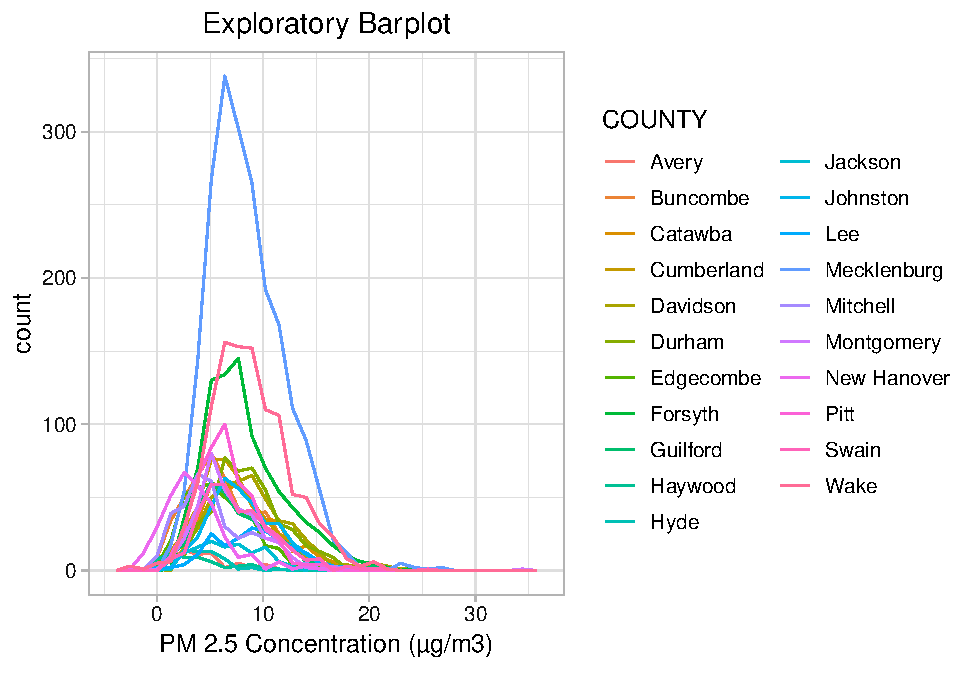
\includegraphics{./Outputunnamed-chunk-11-1.pdf}
\caption{PM2.5 NC 2018 frequency polygon. \label{PM2.5_freqpoly}}
\end{figure}

\begin{figure}
\centering
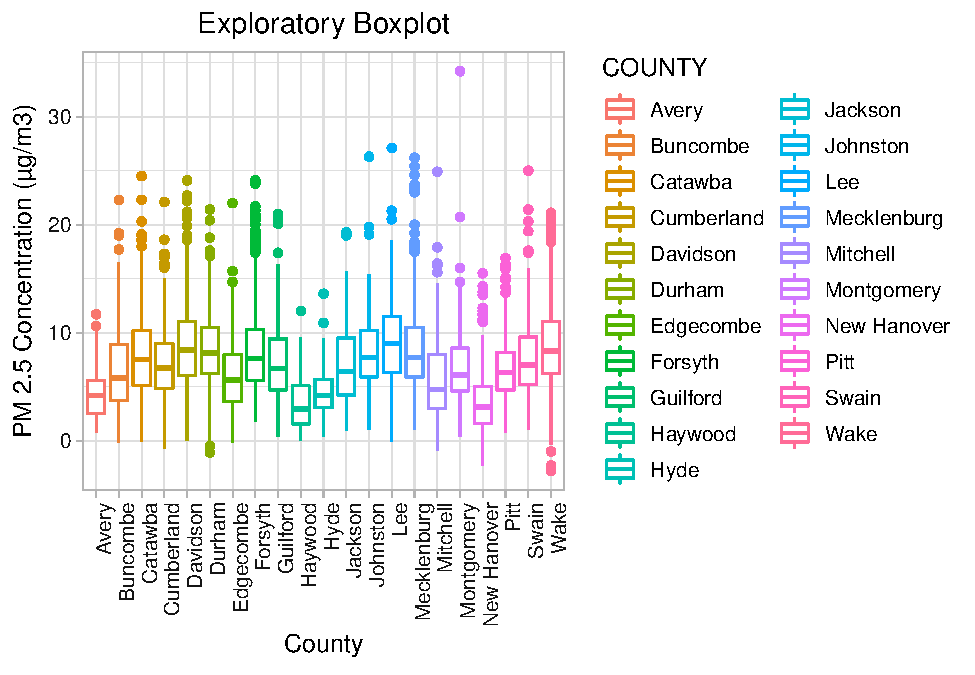
\includegraphics{./Outputunnamed-chunk-12-1.pdf}
\caption{PM2.5 NC 2018 boxplot. \label{PM2.5_boxplot}}
\end{figure}

\begin{figure}
\centering
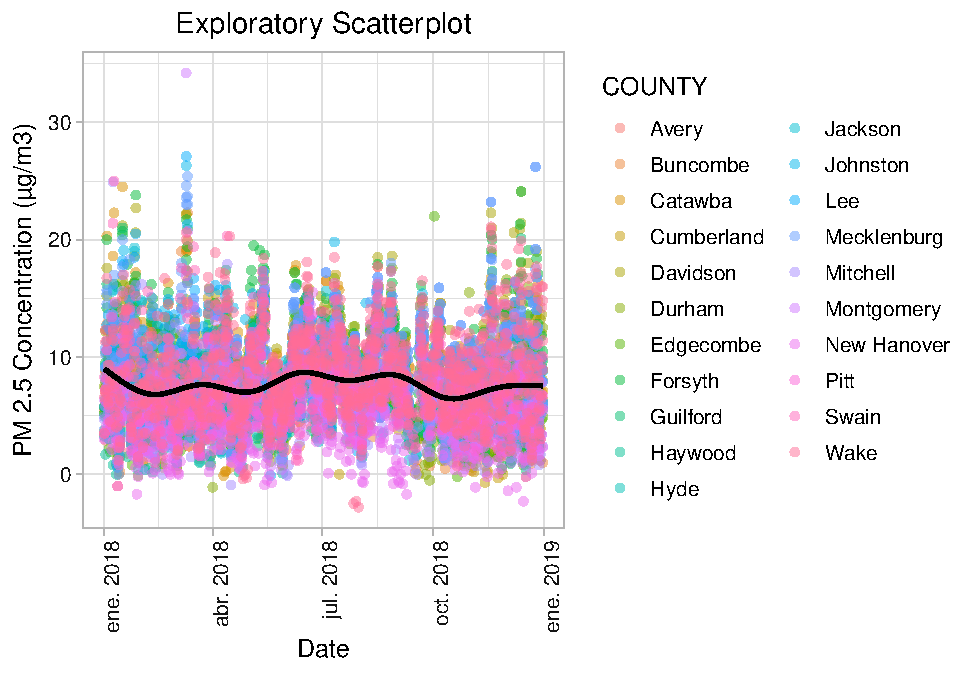
\includegraphics{./Outputunnamed-chunk-13-1.pdf}
\caption{PM2.5 NC 2018 scatterplot. \label{PM2.5_scatterplot}}
\end{figure}

Visual data exploration of the PM10 2018 raw data file in
\autoref{PM10_scatterplot}.

\begin{figure}
\centering
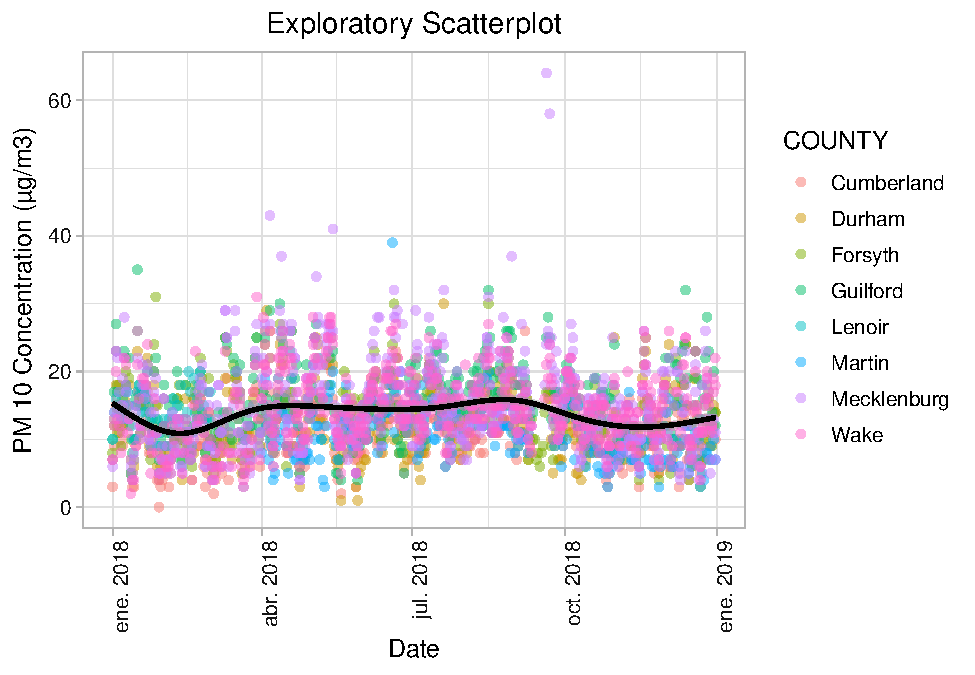
\includegraphics{./Outputunnamed-chunk-14-1.pdf}
\caption{PM10 NC 2018 scatterplot. \label{PM10_scatterplot}}
\end{figure}

Data wrangling of the PM2.5 and PM10 2018 raw data files.

\begin{Shaded}
\begin{Highlighting}[]
\CommentTok{#Selecting Columns}
\NormalTok{EPA_AQ_PM25_NC2018_Temp <-}\StringTok{ }\KeywordTok{select}\NormalTok{(EPA_AQPM25_NC2018_raw, Date, Site.ID,}
\NormalTok{                                Daily.Mean.PM2.}\FloatTok{5.}\NormalTok{Concentration, AQS_PARAMETER_DESC,}
\NormalTok{                                COUNTY}\OperatorTok{:}\NormalTok{SITE_LONGITUDE)}

\CommentTok{#Changing column name}
\KeywordTok{colnames}\NormalTok{(EPA_AQ_PM25_NC2018_Temp)[}\KeywordTok{colnames}\NormalTok{(EPA_AQ_PM25_NC2018_Temp)}
                                \OperatorTok{==}\StringTok{"Daily.Mean.PM2.5.Concentration"}\NormalTok{]<-}\StringTok{"Daily.Mean.Concentration"}

\CommentTok{#Selecting Columns}
\NormalTok{EPA_AQ_PM10_NC2018_Temp <-}\StringTok{ }\KeywordTok{select}\NormalTok{(EPA_AQPM10_NC2018_raw, Date, Site.ID,}
\NormalTok{                                Daily.Mean.PM10.Concentration, AQS_PARAMETER_DESC,}
\NormalTok{                                COUNTY}\OperatorTok{:}\NormalTok{SITE_LONGITUDE)}

\CommentTok{#Changing column name}
\KeywordTok{colnames}\NormalTok{(EPA_AQ_PM10_NC2018_Temp)[}\KeywordTok{colnames}\NormalTok{(EPA_AQ_PM10_NC2018_Temp)}
                                \OperatorTok{==}\StringTok{"Daily.Mean.PM10.Concentration"}\NormalTok{]<-}\StringTok{"Daily.Mean.Concentration"}

\CommentTok{#Create AQS_PARAMETER_DESC Column with Contaminant description.}
\NormalTok{EPA_AQ_PM25_NC2018_Temp}\OperatorTok{$}\NormalTok{AQS_PARAMETER_DESC <-}\StringTok{ "PM2.5"}
\NormalTok{EPA_AQ_PM10_NC2018_Temp}\OperatorTok{$}\NormalTok{AQS_PARAMETER_DESC <-}\StringTok{ "PM10"}

\CommentTok{#Eliminates duplicate dates}
\NormalTok{EPA_AQ_PM25_NC2018_Cleaned <-}\StringTok{ }\NormalTok{EPA_AQ_PM25_NC2018_Temp [}\OperatorTok{!}\KeywordTok{duplicated}\NormalTok{(EPA_AQ_PM25_NC2018_Temp[}\KeywordTok{c}\NormalTok{(}\DecValTok{1}\NormalTok{,}\DecValTok{2}\NormalTok{)]),]}

\NormalTok{EPA_AQ_PM10_NC2018_Cleaned <-}\StringTok{ }\NormalTok{EPA_AQ_PM10_NC2018_Temp [}\OperatorTok{!}\KeywordTok{duplicated}\NormalTok{(EPA_AQ_PM10_NC2018_Temp[}\KeywordTok{c}\NormalTok{(}\DecValTok{1}\NormalTok{,}\DecValTok{2}\NormalTok{)]),]}

\CommentTok{# Combine the data.}
\NormalTok{EPA_AQ_PM2.5PM10_NC2018_Cleaned <-}\StringTok{ }\KeywordTok{rbind}\NormalTok{(EPA_AQ_PM25_NC2018_Cleaned, EPA_AQ_PM10_NC2018_Cleaned)}

\CommentTok{#Save the data in the processed folder}
\KeywordTok{write.csv}\NormalTok{(EPA_AQ_PM2.5PM10_NC2018_Cleaned,}
         \StringTok{"./Data/Processed/EPA_AQ_PM2.5PM10_NC2018_Cleaned.csv"}\NormalTok{)}

\CommentTok{#Spread PM2.5 and PM10}
\NormalTok{EPA_AQ_PM2.5PM10_NC2018_Spread <-}\StringTok{ }
\StringTok{  }\NormalTok{EPA_AQ_PM2.5PM10_NC2018_Cleaned }\OperatorTok
\StringTok{  }\KeywordTok{spread}\NormalTok{(AQS_PARAMETER_DESC, Daily.Mean.Concentration)}

\CommentTok{#Remove rows without PM2.5 data}
\NormalTok{EPA_AQ_PM2.5PM10_NC2018_Spread <-}\StringTok{ }\NormalTok{EPA_AQ_PM2.5PM10_NC2018_Spread[}\OperatorTok{!}\KeywordTok{is.na}\NormalTok{(EPA_AQ_PM2.5PM10_NC2018_Spread}\OperatorTok{$}\NormalTok{PM2.}\DecValTok{5}\NormalTok{),]}

\CommentTok{#Convert the dataset to a spatially enabled "sf" data frame}
\NormalTok{PM2.5_PM10_sf <-}\StringTok{ }\KeywordTok{st_as_sf}\NormalTok{(EPA_AQ_PM2.5PM10_NC2018_Spread,}\DataTypeTok{coords =} \KeywordTok{c}\NormalTok{(}\StringTok{'SITE_LONGITUDE'}\NormalTok{,}\StringTok{'SITE_LATITUDE'}\NormalTok{),}\DataTypeTok{crs=}\DecValTok{4269}\NormalTok{)}

\CommentTok{#Convert all to UTM Zone 17 (crs = 26917)}
\NormalTok{PM2.5_PM10_sf_utm <-}\StringTok{ }\KeywordTok{st_transform}\NormalTok{(PM2.5_PM10_sf, }\DataTypeTok{c=}\DecValTok{26917}\NormalTok{)}
\end{Highlighting}
\end{Shaded}

In \autoref{PM2.5Stations} is presented the locations of the PM2.5
monitoring stations.

\begin{figure}
\centering
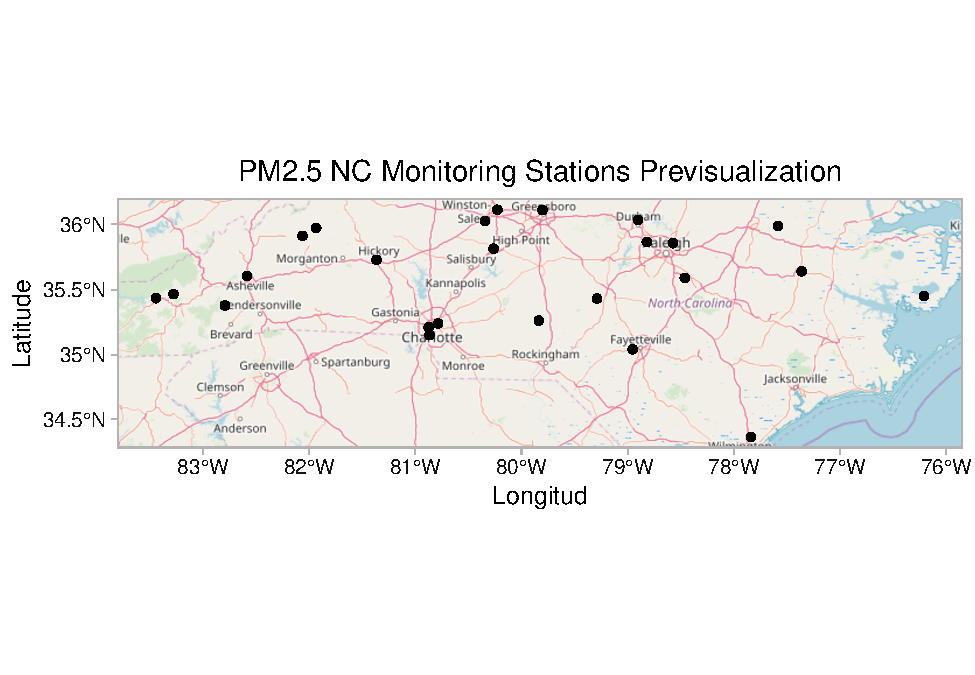
\includegraphics{./Outputunnamed-chunk-16-1.pdf}
\caption{PM2.5 NC Monitoring Stations Previsualization.
\label{PM2.5Stations}}
\end{figure}

\subsection{North Carolina Counties Zoning, Geographic information, and
Population
Data}\label{north-carolina-counties-zoning-geographic-information-and-population-data}

Downloading the list of North Carolina Counties and Population from a
Wikipedia URL.

\begin{Shaded}
\begin{Highlighting}[]
\CommentTok{#North Carolina Counties}
\NormalTok{url <-}\StringTok{ "https://en.wikipedia.org/wiki/List_of_counties_in_North_Carolina"}
\NormalTok{webpage <-}\StringTok{ }\KeywordTok{read_html}\NormalTok{(url)}

\NormalTok{County_Name <-}\StringTok{ }\NormalTok{webpage }\OperatorTok\StringTok{ }\KeywordTok{html_nodes}\NormalTok{(}\StringTok{"th:nth-child(1)"}\NormalTok{) }\OperatorTok\StringTok{ }\KeywordTok{html_text}\NormalTok{()}
\NormalTok{County_Population <-}\StringTok{ }\NormalTok{webpage }\OperatorTok\StringTok{ }\KeywordTok{html_nodes}\NormalTok{(}\StringTok{"tr :nth-child(7)"}\NormalTok{) }\OperatorTok\StringTok{ }\KeywordTok{html_text}\NormalTok{() }

\CommentTok{#Remove unwanted info and characters}
\NormalTok{County_Info <-}\StringTok{ }\KeywordTok{data_frame}\NormalTok{(}\DataTypeTok{County =}\NormalTok{ County_Name[}\DecValTok{9}\OperatorTok{:}\DecValTok{108}\NormalTok{])}
\NormalTok{County_Info}\OperatorTok{$}\NormalTok{County <-}\StringTok{ }\KeywordTok{str_replace}\NormalTok{(County_Info}\OperatorTok{$}\NormalTok{County, }\StringTok{" County"}\NormalTok{, }\StringTok{""}\NormalTok{)}
\NormalTok{County_Info}\OperatorTok{$}\NormalTok{County <-}\StringTok{ }\KeywordTok{str_replace}\NormalTok{(County_Info}\OperatorTok{$}\NormalTok{County, }\StringTok{"}\CharTok{\textbackslash{}n}\StringTok{"}\NormalTok{, }\StringTok{""}\NormalTok{)}

\NormalTok{Population <-}\StringTok{ }\KeywordTok{data_frame}\NormalTok{(}\DataTypeTok{Population=}\NormalTok{County_Population[}\DecValTok{2}\OperatorTok{:}\DecValTok{101}\NormalTok{])}

\NormalTok{County_Info <-}\StringTok{ }\KeywordTok{cbind}\NormalTok{(County_Info, Population)}

\NormalTok{County_Info}\OperatorTok{$}\NormalTok{Population <-}\StringTok{ }\KeywordTok{str_replace}\NormalTok{(County_Info}\OperatorTok{$}\NormalTok{Population,}\StringTok{","}\NormalTok{,}\StringTok{""}\NormalTok{)}
\NormalTok{County_Info}\OperatorTok{$}\NormalTok{Population <-}\StringTok{ }\KeywordTok{str_replace}\NormalTok{(County_Info}\OperatorTok{$}\NormalTok{Population,}\StringTok{","}\NormalTok{,}\StringTok{""}\NormalTok{)}

\NormalTok{County_Info}\OperatorTok{$}\NormalTok{Population <-}\StringTok{ }\KeywordTok{as.numeric}\NormalTok{(County_Info}\OperatorTok{$}\NormalTok{Population) }
\end{Highlighting}
\end{Shaded}

Assigning the corresponding zone to each county. Info from: Rudersdorf,
Amy. 2010. ``NC County Maps.'' Government \& Heritage Library, State
Library of North Carolina.

\begin{Shaded}
\begin{Highlighting}[]
\CommentTok{#North Carolina Zones}
\NormalTok{County_Info}\OperatorTok{$}\NormalTok{Zone<-}\KeywordTok{ifelse}\NormalTok{(County_Info}\OperatorTok{$}\NormalTok{County }\OperatorTok{==}\StringTok{ 'Ashe'}\OperatorTok{|}\NormalTok{County_Info}\OperatorTok{$}\NormalTok{County }\OperatorTok{==}\StringTok{'Alleghany'}\OperatorTok{|}\NormalTok{County_Info}\OperatorTok{$}\NormalTok{County }\OperatorTok{==}\StringTok{'Wilkes'}\OperatorTok{|}\NormalTok{County_Info}\OperatorTok{$}\NormalTok{County }\OperatorTok{==}\StringTok{'Watauga'}\OperatorTok{|}\NormalTok{County_Info}\OperatorTok{$}\NormalTok{County }\OperatorTok{==}\StringTok{'Avery'}\OperatorTok{|}\NormalTok{County_Info}\OperatorTok{$}\NormalTok{County }\OperatorTok{==}\StringTok{'Caldwell'}\OperatorTok{|}\NormalTok{County_Info}\OperatorTok{$}\NormalTok{County }\OperatorTok{==}\StringTok{'Mitchell'}\OperatorTok{|}\NormalTok{County_Info}\OperatorTok{$}\NormalTok{County }\OperatorTok{==}\StringTok{'Burke'}\OperatorTok{|}\NormalTok{County_Info}\OperatorTok{$}\NormalTok{County }\OperatorTok{==}\StringTok{'Yancey'}\OperatorTok{|}\NormalTok{County_Info}\OperatorTok{$}\NormalTok{County }\OperatorTok{==}\StringTok{'McDowell'}\OperatorTok{|}\NormalTok{County_Info}\OperatorTok{$}\NormalTok{County }\OperatorTok{==}\StringTok{'Rutherford'}\OperatorTok{|}\NormalTok{County_Info}\OperatorTok{$}\NormalTok{County }\OperatorTok{==}\StringTok{'Madison'}\OperatorTok{|}\NormalTok{County_Info}\OperatorTok{$}\NormalTok{County }\OperatorTok{==}\StringTok{'Buncombe'}\OperatorTok{|}\NormalTok{County_Info}\OperatorTok{$}\NormalTok{County }\OperatorTok{==}\StringTok{'Polk'}\OperatorTok{|}\NormalTok{County_Info}\OperatorTok{$}\NormalTok{County }\OperatorTok{==}\StringTok{'Henderson'}\OperatorTok{|}\NormalTok{County_Info}\OperatorTok{$}\NormalTok{County }\OperatorTok{==}\StringTok{'Haywood'}\OperatorTok{|}\NormalTok{County_Info}\OperatorTok{$}\NormalTok{County }\OperatorTok{==}\StringTok{'Transylvania'}\OperatorTok{|}\NormalTok{County_Info}\OperatorTok{$}\NormalTok{County }\OperatorTok{==}\StringTok{'Swain'}\OperatorTok{|}\NormalTok{County_Info}\OperatorTok{$}\NormalTok{County }\OperatorTok{==}\StringTok{'Jackson'}\OperatorTok{|}\NormalTok{County_Info}\OperatorTok{$}\NormalTok{County }\OperatorTok{==}\StringTok{'Graham'}\OperatorTok{|}\NormalTok{County_Info}\OperatorTok{$}\NormalTok{County }\OperatorTok{==}\StringTok{'Macon'}\OperatorTok{|}\NormalTok{County_Info}\OperatorTok{$}\NormalTok{County }\OperatorTok{==}\StringTok{'Cherokee'}\OperatorTok{|}\NormalTok{County_Info}\OperatorTok{$}\NormalTok{County }\OperatorTok{==}\StringTok{'Clay'}\NormalTok{,}\StringTok{'Mountains'}\NormalTok{,}
                         \KeywordTok{ifelse}\NormalTok{(County_Info}\OperatorTok{$}\NormalTok{County }\OperatorTok{==}\StringTok{ 'Surry'}\OperatorTok{|}\NormalTok{County_Info}\OperatorTok{$}\NormalTok{County }\OperatorTok{==}\StringTok{'Stokes'}\OperatorTok{|}\NormalTok{County_Info}\OperatorTok{$}\NormalTok{County }\OperatorTok{==}\StringTok{'Rockingham'}\OperatorTok{|}\NormalTok{County_Info}\OperatorTok{$}\NormalTok{County }\OperatorTok{==}\StringTok{'Caswell'}\OperatorTok{|}\NormalTok{County_Info}\OperatorTok{$}\NormalTok{County }\OperatorTok{==}\StringTok{'Person'}\OperatorTok{|}\NormalTok{County_Info}\OperatorTok{$}\NormalTok{County }\OperatorTok{==}\StringTok{'Granville'}\OperatorTok{|}\NormalTok{County_Info}\OperatorTok{$}\NormalTok{County }\OperatorTok{==}\StringTok{'Vance'}\OperatorTok{|}\NormalTok{County_Info}\OperatorTok{$}\NormalTok{County }\OperatorTok{==}\StringTok{'Warren'}\OperatorTok{|}\NormalTok{County_Info}\OperatorTok{$}\NormalTok{County }\OperatorTok{==}\StringTok{'Yadkin'}\OperatorTok{|}\NormalTok{County_Info}\OperatorTok{$}\NormalTok{County }\OperatorTok{==}\StringTok{'Forsyth'}\OperatorTok{|}\NormalTok{County_Info}\OperatorTok{$}\NormalTok{County }\OperatorTok{==}\StringTok{'Guilford'}\OperatorTok{|}\NormalTok{County_Info}\OperatorTok{$}\NormalTok{County }\OperatorTok{==}\StringTok{'Alamance'}\OperatorTok{|}\NormalTok{County_Info}\OperatorTok{$}\NormalTok{County }\OperatorTok{==}\StringTok{'Orange'}\OperatorTok{|}\NormalTok{County_Info}\OperatorTok{$}\NormalTok{County }\OperatorTok{==}\StringTok{'Durham'}\OperatorTok{|}\NormalTok{County_Info}\OperatorTok{$}\NormalTok{County }\OperatorTok{==}\StringTok{'Franklin'}\OperatorTok{|}\NormalTok{County_Info}\OperatorTok{$}\NormalTok{County }\OperatorTok{==}\StringTok{'Alexander'}\OperatorTok{|}\NormalTok{County_Info}\OperatorTok{$}\NormalTok{County }\OperatorTok{==}\StringTok{'Iredell'}\OperatorTok{|}\NormalTok{County_Info}\OperatorTok{$}\NormalTok{County }\OperatorTok{==}\StringTok{'Davie'}\OperatorTok{|}\NormalTok{County_Info}\OperatorTok{$}\NormalTok{County }\OperatorTok{==}\StringTok{'Rowan'}\OperatorTok{|}\NormalTok{County_Info}\OperatorTok{$}\NormalTok{County }\OperatorTok{==}\StringTok{'Davidson'}\OperatorTok{|}\NormalTok{County_Info}\OperatorTok{$}\NormalTok{County }\OperatorTok{==}\StringTok{'Randolph'}\OperatorTok{|}\NormalTok{County_Info}\OperatorTok{$}\NormalTok{County }\OperatorTok{==}\StringTok{'Chatham'}\OperatorTok{|}\NormalTok{County_Info}\OperatorTok{$}\NormalTok{County }\OperatorTok{==}\StringTok{'Wake'}\OperatorTok{|}\NormalTok{County_Info}\OperatorTok{$}\NormalTok{County }\OperatorTok{==}\StringTok{'Catawba'}\OperatorTok{|}\NormalTok{County_Info}\OperatorTok{$}\NormalTok{County }\OperatorTok{==}\StringTok{'Cleveland'}\OperatorTok{|}\NormalTok{County_Info}\OperatorTok{$}\NormalTok{County }\OperatorTok{==}\StringTok{'Lincoln'}\OperatorTok{|}\NormalTok{County_Info}\OperatorTok{$}\NormalTok{County }\OperatorTok{==}\StringTok{'Gaston'}\OperatorTok{|}\NormalTok{County_Info}\OperatorTok{$}\NormalTok{County }\OperatorTok{==}\StringTok{'Mecklenburg'}\OperatorTok{|}\NormalTok{County_Info}\OperatorTok{$}\NormalTok{County }\OperatorTok{==}\StringTok{'Cabarrus'}\OperatorTok{|}\NormalTok{County_Info}\OperatorTok{$}\NormalTok{County }\OperatorTok{==}\StringTok{'Stanly'}\OperatorTok{|}\NormalTok{County_Info}\OperatorTok{$}\NormalTok{County }\OperatorTok{==}\StringTok{'Union'}\OperatorTok{|}\NormalTok{County_Info}\OperatorTok{$}\NormalTok{County }\OperatorTok{==}\StringTok{'Montgomery'}\OperatorTok{|}\NormalTok{County_Info}\OperatorTok{$}\NormalTok{County }\OperatorTok{==}\StringTok{'Anson'}\OperatorTok{|}\NormalTok{County_Info}\OperatorTok{$}\NormalTok{County }\OperatorTok{==}\StringTok{'Moore'}\OperatorTok{|}\NormalTok{County_Info}\OperatorTok{$}\NormalTok{County }\OperatorTok{==}\StringTok{'Lee'}\OperatorTok{|}\NormalTok{County_Info}\OperatorTok{$}\NormalTok{County }\OperatorTok{==}\StringTok{'Richmond'}\NormalTok{,}\StringTok{'Piedmont'}\NormalTok{,}
                                \KeywordTok{ifelse}\NormalTok{(County_Info}\OperatorTok{$}\NormalTok{County }\OperatorTok{==}\StringTok{ 'Scotland'}\OperatorTok{|}\NormalTok{County_Info}\OperatorTok{$}\NormalTok{County }\OperatorTok{==}\StringTok{'Hoke'}\OperatorTok{|}\NormalTok{County_Info}\OperatorTok{$}\NormalTok{County }\OperatorTok{==}\StringTok{'Harnett'}\OperatorTok{|}\NormalTok{County_Info}\OperatorTok{$}\NormalTok{County }\OperatorTok{==}\StringTok{'Johnston'}\OperatorTok{|}\NormalTok{County_Info}\OperatorTok{$}\NormalTok{County }\OperatorTok{==}\StringTok{'Nash'}\OperatorTok{|}\NormalTok{County_Info}\OperatorTok{$}\NormalTok{County }\OperatorTok{==}\StringTok{'Halifax'}\OperatorTok{|}\NormalTok{County_Info}\OperatorTok{$}\NormalTok{County }\OperatorTok{==}\StringTok{'Northampton'}\OperatorTok{|}\NormalTok{County_Info}\OperatorTok{$}\NormalTok{County }\OperatorTok{==}\StringTok{'Robeson'}\OperatorTok{|}\NormalTok{County_Info}\OperatorTok{$}\NormalTok{County }\OperatorTok{==}\StringTok{'Cumberland'}\OperatorTok{|}\NormalTok{County_Info}\OperatorTok{$}\NormalTok{County }\OperatorTok{==}\StringTok{'Sampson'}\OperatorTok{|}\NormalTok{County_Info}\OperatorTok{$}\NormalTok{County }\OperatorTok{==}\StringTok{'Wayne'}\OperatorTok{|}\NormalTok{County_Info}\OperatorTok{$}\NormalTok{County }\OperatorTok{==}\StringTok{'Wilson'}\OperatorTok{|}\NormalTok{County_Info}\OperatorTok{$}\NormalTok{County }\OperatorTok{==}\StringTok{'Edgecombe'}\OperatorTok{|}\NormalTok{County_Info}\OperatorTok{$}\NormalTok{County }\OperatorTok{==}\StringTok{'Columbus'}\OperatorTok{|}\NormalTok{County_Info}\OperatorTok{$}\NormalTok{County }\OperatorTok{==}\StringTok{'Bladen'}\OperatorTok{|}\NormalTok{County_Info}\OperatorTok{$}\NormalTok{County }\OperatorTok{==}\StringTok{'Brunswick'}\OperatorTok{|}\NormalTok{County_Info}\OperatorTok{$}\NormalTok{County }\OperatorTok{==}\StringTok{'New Hanover'}\OperatorTok{|}\NormalTok{County_Info}\OperatorTok{$}\NormalTok{County }\OperatorTok{==}\StringTok{'Pender'}\OperatorTok{|}\NormalTok{County_Info}\OperatorTok{$}\NormalTok{County }\OperatorTok{==}\StringTok{'Duplin'}\OperatorTok{|}\NormalTok{County_Info}\OperatorTok{$}\NormalTok{County }\OperatorTok{==}\StringTok{'Onslow'}\OperatorTok{|}\NormalTok{County_Info}\OperatorTok{$}\NormalTok{County }\OperatorTok{==}\StringTok{'Lenoir'}\OperatorTok{|}\NormalTok{County_Info}\OperatorTok{$}\NormalTok{County }\OperatorTok{==}\StringTok{'Jones'}\OperatorTok{|}\NormalTok{County_Info}\OperatorTok{$}\NormalTok{County }\OperatorTok{==}\StringTok{'Carteret'}\OperatorTok{|}\NormalTok{County_Info}\OperatorTok{$}\NormalTok{County }\OperatorTok{==}\StringTok{'Greene'}\OperatorTok{|}\NormalTok{County_Info}\OperatorTok{$}\NormalTok{County }\OperatorTok{==}\StringTok{'Craven'}\OperatorTok{|}\NormalTok{County_Info}\OperatorTok{$}\NormalTok{County }\OperatorTok{==}\StringTok{'Pitt'}\OperatorTok{|}\NormalTok{County_Info}\OperatorTok{$}\NormalTok{County }\OperatorTok{==}\StringTok{'Pamlico'}\OperatorTok{|}\NormalTok{County_Info}\OperatorTok{$}\NormalTok{County }\OperatorTok{==}\StringTok{'Beaufort'}\OperatorTok{|}\NormalTok{County_Info}\OperatorTok{$}\NormalTok{County }\OperatorTok{==}\StringTok{'Martin'}\OperatorTok{|}\NormalTok{County_Info}\OperatorTok{$}\NormalTok{County }\OperatorTok{==}\StringTok{'Bertie'}\OperatorTok{|}\NormalTok{County_Info}\OperatorTok{$}\NormalTok{County }\OperatorTok{==}\StringTok{'Hyde'}\OperatorTok{|}\NormalTok{County_Info}\OperatorTok{$}\NormalTok{County }\OperatorTok{==}\StringTok{'Dare'}\OperatorTok{|}\NormalTok{County_Info}\OperatorTok{$}\NormalTok{County }\OperatorTok{==}\StringTok{'Tyrrell'}\OperatorTok{|}\NormalTok{County_Info}\OperatorTok{$}\NormalTok{County }\OperatorTok{==}\StringTok{'Washington'}\OperatorTok{|}\NormalTok{County_Info}\OperatorTok{$}\NormalTok{County }\OperatorTok{==}\StringTok{'Hertford'}\OperatorTok{|}\NormalTok{County_Info}\OperatorTok{$}\NormalTok{County }\OperatorTok{==}\StringTok{'Gates'}\OperatorTok{|}\NormalTok{County_Info}\OperatorTok{$}\NormalTok{County }\OperatorTok{==}\StringTok{'Currituck'}\OperatorTok{|}\NormalTok{County_Info}\OperatorTok{$}\NormalTok{County }\OperatorTok{==}\StringTok{'Camden'}\OperatorTok{|}\NormalTok{County_Info}\OperatorTok{$}\NormalTok{County }\OperatorTok{==}\StringTok{'Pasquotank'}\OperatorTok{|}\NormalTok{County_Info}\OperatorTok{$}\NormalTok{County }\OperatorTok{==}\StringTok{'Perquimans'}\OperatorTok{|}\NormalTok{County_Info}\OperatorTok{$}\NormalTok{County }\OperatorTok{==}\StringTok{'Chowan'}\NormalTok{,}\StringTok{'Coastal'}\NormalTok{,}\StringTok{'NoInfo'}\NormalTok{)))}
\end{Highlighting}
\end{Shaded}

Data exploration of the County\_Info dataframe.

\begin{Shaded}
\begin{Highlighting}[]
\KeywordTok{dim}\NormalTok{(County_Info)}
\end{Highlighting}
\end{Shaded}

\begin{verbatim}
## [1] 100   3
\end{verbatim}

\begin{Shaded}
\begin{Highlighting}[]
\KeywordTok{str}\NormalTok{(County_Info)}
\end{Highlighting}
\end{Shaded}

\begin{verbatim}
## 'data.frame':    100 obs. of  3 variables:
##  $ County    : chr  "Alamance" "Alexander" "Alleghany" "Anson" ...
##  $ Population: num  157844 37159 10935 25531 26833 ...
##  $ Zone      : chr  "Piedmont" "Piedmont" "Mountains" "Piedmont" ...
\end{verbatim}

\begin{Shaded}
\begin{Highlighting}[]
\KeywordTok{colnames}\NormalTok{(County_Info)}
\end{Highlighting}
\end{Shaded}

\begin{verbatim}
## [1] "County"     "Population" "Zone"
\end{verbatim}

\begin{Shaded}
\begin{Highlighting}[]
\KeywordTok{summary}\NormalTok{(County_Info)}
\end{Highlighting}
\end{Shaded}

\begin{verbatim}
##     County            Population          Zone          
##  Length:100         Min.   :   4090   Length:100        
##  Class :character   1st Qu.:  25001   Class :character  
##  Mode  :character   Median :  55311   Mode  :character  
##                     Mean   : 100526                     
##                     3rd Qu.: 114764                     
##                     Max.   :1034290
\end{verbatim}

\begin{Shaded}
\begin{Highlighting}[]
\KeywordTok{unique}\NormalTok{(County_Info}\OperatorTok{$}\NormalTok{Zone)}
\end{Highlighting}
\end{Shaded}

\begin{verbatim}
## [1] "Piedmont"  "Mountains" "Coastal"
\end{verbatim}

Adding the County Information to the PM2.5\_PM10\_sf\_utm dataframe.

\begin{Shaded}
\begin{Highlighting}[]
\NormalTok{PM2.5_PM10_Info_sf_utm <-}\StringTok{ }\NormalTok{PM2.5_PM10_sf_utm }\OperatorTok
\KeywordTok{left_join}\NormalTok{(County_Info, }\DataTypeTok{by =} \KeywordTok{c}\NormalTok{(}\StringTok{"COUNTY"}\NormalTok{=}\StringTok{"County"}\NormalTok{))}
\end{Highlighting}
\end{Shaded}

\subsection{US Census Bureau US counties
shapefile}\label{us-census-bureau-us-counties-shapefile-1}

Reading the USA county shapefile, sub-setting for NC.

\begin{Shaded}
\begin{Highlighting}[]
\NormalTok{counties_sf<-}\StringTok{ }\KeywordTok{st_read}\NormalTok{(}\StringTok{'./Data/Spatial/cb_2017_us_county_20m.shp'}\NormalTok{) }\OperatorTok\StringTok{ }
\StringTok{  }\KeywordTok{filter}\NormalTok{(STATEFP }\OperatorTok{==}\StringTok{ }\DecValTok{37}\NormalTok{) }\CommentTok{#Filter for just NC Counties}
\end{Highlighting}
\end{Shaded}

\begin{verbatim}
## Reading layer `cb_2017_us_county_20m' from data source `C:\Users\Felipe\OneDrive - Duke University\1. DUKE\1. Ramos 2 Semestre\EOS-872 Env. Data Analytics\DataAnalytics_FinalProject\Data\Spatial\cb_2017_us_county_20m.shp' using driver `ESRI Shapefile'
## Simple feature collection with 3220 features and 9 fields
## geometry type:  MULTIPOLYGON
## dimension:      XY
## bbox:           xmin: -179.1743 ymin: 17.91377 xmax: 179.7739 ymax: 71.35256
## epsg (SRID):    4269
## proj4string:    +proj=longlat +datum=NAD83 +no_defs
\end{verbatim}

\begin{Shaded}
\begin{Highlighting}[]
\CommentTok{#CRS}
\KeywordTok{st_crs}\NormalTok{(counties_sf) }\CommentTok{#crs=4269 = NAD83.}
\end{Highlighting}
\end{Shaded}

\begin{verbatim}
## Coordinate Reference System:
##   EPSG: 4269 
##   proj4string: "+proj=longlat +datum=NAD83 +no_defs"
\end{verbatim}

Converting the counties\_sf to UTM Zone 17

\begin{Shaded}
\begin{Highlighting}[]
\CommentTok{#Convert all to UTM Zone 17 (crs = 26917)}
\NormalTok{counties_sf_utm <-}\StringTok{ }\KeywordTok{st_transform}\NormalTok{(counties_sf, }\DataTypeTok{c=}\DecValTok{26917}\NormalTok{)}

\CommentTok{#Adding the Zone Info}
\NormalTok{counties_sf_utm <-}\StringTok{ }\NormalTok{counties_sf_utm }\OperatorTok
\KeywordTok{left_join}\NormalTok{(County_Info, }\DataTypeTok{by =} \KeywordTok{c}\NormalTok{(}\StringTok{"NAME"}\NormalTok{=}\StringTok{"County"}\NormalTok{))}
\end{Highlighting}
\end{Shaded}

Data exploration of the County\_Info dataframe.

\begin{Shaded}
\begin{Highlighting}[]
\KeywordTok{dim}\NormalTok{(counties_sf_utm)}
\end{Highlighting}
\end{Shaded}

\begin{verbatim}
## [1] 100  12
\end{verbatim}

\begin{Shaded}
\begin{Highlighting}[]
\KeywordTok{str}\NormalTok{(counties_sf_utm)}
\end{Highlighting}
\end{Shaded}

\begin{verbatim}
## Classes 'sf' and 'data.frame':   100 obs. of  12 variables:
##  $ STATEFP   : Factor w/ 52 levels "01","02","04",..: 34 34 34 34 34 34 34 34 34 34 ...
##  $ COUNTYFP  : Factor w/ 325 levels "001","003","005",..: 116 71 94 54 62 125 84 102 26 19 ...
##  $ COUNTYNS  : Factor w/ 3220 levels "00023901","00025441",..: 1672 1649 1659 1639 1644 1677 1700 1664 1625 1622 ...
##  $ AFFGEOID  : Factor w/ 3220 levels "0500000US01001",..: 1981 1944 1964 1931 1937 1988 1955 1970 1909 1904 ...
##  $ GEOID     : Factor w/ 3220 levels "01001","01003",..: 1981 1944 1964 1931 1937 1988 1955 1970 1909 1904 ...
##  $ NAME      : chr  "Vance" "Lenoir" "Pitt" "Guilford" ...
##  $ LSAD      : Factor w/ 9 levels "00","03","04",..: 5 5 5 5 5 5 5 5 5 5 ...
##  $ ALAND     : num  6.54e+08 1.03e+09 1.69e+09 1.67e+09 1.01e+09 ...
##  $ AWATER    : num  42187365 5900300 8248766 30723331 3981006 ...
##  $ Population: num  44420 57934 176484 517197 52571 ...
##  $ Zone      : chr  "Piedmont" "Coastal" "Coastal" "Piedmont" ...
##  $ geometry  :sfc_MULTIPOLYGON of length 100; first list element: List of 1
##   ..$ :List of 1
##   .. ..$ : num [1:10, 1:2] 724066 727615 739570 744478 741926 ...
##   ..- attr(*, "class")= chr  "XY" "MULTIPOLYGON" "sfg"
##  - attr(*, "sf_column")= chr "geometry"
##  - attr(*, "agr")= Factor w/ 3 levels "constant","aggregate",..: NA NA NA NA NA NA NA NA NA NA ...
##   ..- attr(*, "names")= chr  "STATEFP" "COUNTYFP" "COUNTYNS" "AFFGEOID" ...
\end{verbatim}

\begin{Shaded}
\begin{Highlighting}[]
\KeywordTok{colnames}\NormalTok{(counties_sf_utm)}
\end{Highlighting}
\end{Shaded}

\begin{verbatim}
##  [1] "STATEFP"    "COUNTYFP"   "COUNTYNS"   "AFFGEOID"   "GEOID"     
##  [6] "NAME"       "LSAD"       "ALAND"      "AWATER"     "Population"
## [11] "Zone"       "geometry"
\end{verbatim}

\begin{Shaded}
\begin{Highlighting}[]
\KeywordTok{summary}\NormalTok{(counties_sf_utm)}
\end{Highlighting}
\end{Shaded}

\begin{verbatim}
##     STATEFP       COUNTYFP      COUNTYNS            AFFGEOID      GEOID   
##  37     :100   001    : 1   01008531: 1   0500000US37001: 1   37001  : 1  
##  01     :  0   003    : 1   01008532: 1   0500000US37003: 1   37003  : 1  
##  02     :  0   005    : 1   01008533: 1   0500000US37005: 1   37005  : 1  
##  04     :  0   007    : 1   01008534: 1   0500000US37007: 1   37007  : 1  
##  05     :  0   009    : 1   01008535: 1   0500000US37009: 1   37009  : 1  
##  06     :  0   011    : 1   01008536: 1   0500000US37011: 1   37011  : 1  
##  (Other):  0   (Other):94   (Other) :94   (Other)       :94   (Other):94  
##      NAME                LSAD         ALAND               AWATER         
##  Length:100         06     :100   Min.   :4.472e+08   Min.   :4.453e+05  
##  Class :character   00     :  0   1st Qu.:8.936e+08   1st Qu.:7.287e+06  
##  Mode  :character   03     :  0   Median :1.192e+09   Median :1.595e+07  
##                     04     :  0   Mean   :1.259e+09   Mean   :1.347e+08  
##                     05     :  0   3rd Qu.:1.501e+09   3rd Qu.:3.831e+07  
##                     12     :  0   Max.   :2.453e+09   Max.   :3.001e+09  
##                     (Other):  0                                          
##    Population          Zone                    geometry  
##  Min.   :   4090   Length:100         MULTIPOLYGON :100  
##  1st Qu.:  25001   Class :character   epsg:26917   :  0  
##  Median :  55311   Mode  :character   +proj=utm ...:  0  
##  Mean   : 100526                                         
##  3rd Qu.: 114764                                         
##  Max.   :1034290                                         
## 
\end{verbatim}

Visual data exploration of the counties\_sf\_utm dataframe in
\autoref{Countyplot}.

\begin{figure}
\centering
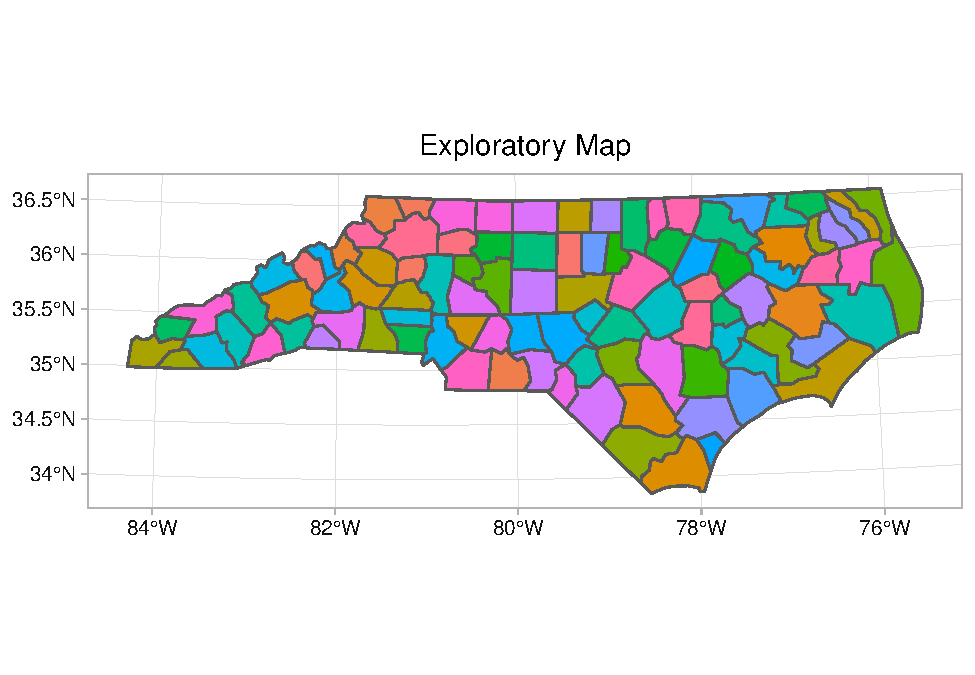
\includegraphics{./Outputunnamed-chunk-23-1.pdf}
\caption{Counties exploratory map. \label{Countyplot}}
\end{figure}

\begin{figure}
\centering
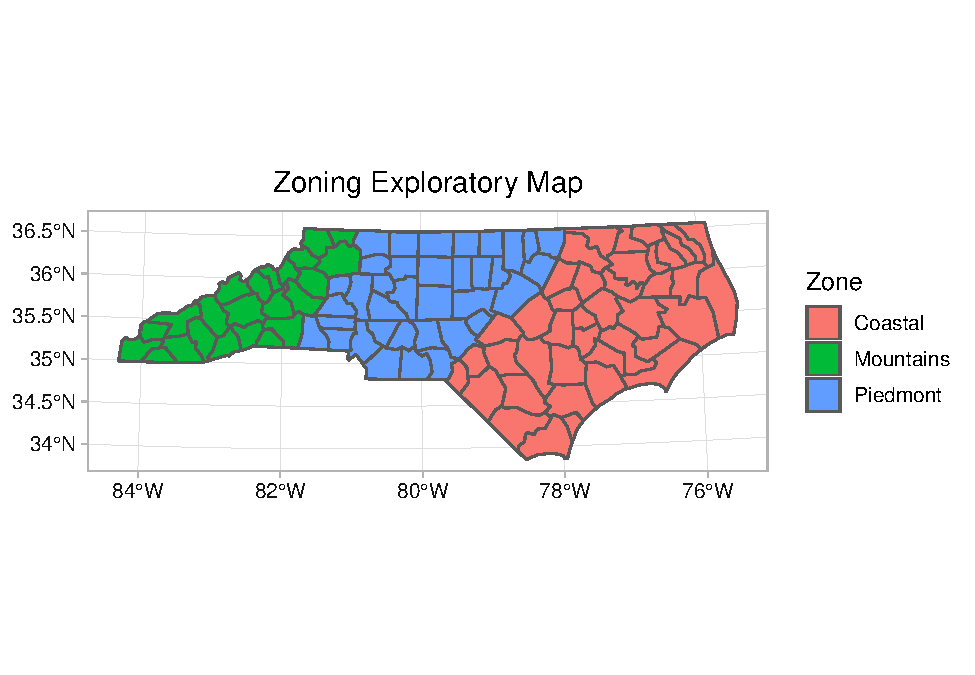
\includegraphics{./Outputunnamed-chunk-24-1.pdf}
\caption{NC Zoning exploratory map. \label{Zoneplot}}
\end{figure}

\subsection{NOAA Average Temperature
Dataset}\label{noaa-average-temperature-dataset-1}

Reading the 2018 North Carolina Air Temperature data.

\begin{Shaded}
\begin{Highlighting}[]
\CommentTok{#Read the 2018 Air Temperature data}
\NormalTok{NOAA_DTAVG_NC2018_raw <-}\StringTok{ }\KeywordTok{read.csv}\NormalTok{(}\StringTok{"./Data/Raw/NOAA_TAVG_NC2018_raw.csv"}\NormalTok{)}
\end{Highlighting}
\end{Shaded}

Data exploration of the NOAA\_DTAVG\_NC2018\_raw dataframe.

\begin{Shaded}
\begin{Highlighting}[]
\KeywordTok{dim}\NormalTok{(NOAA_DTAVG_NC2018_raw)}
\end{Highlighting}
\end{Shaded}

\begin{verbatim}
## [1] 283423      7
\end{verbatim}

\begin{Shaded}
\begin{Highlighting}[]
\KeywordTok{str}\NormalTok{(NOAA_DTAVG_NC2018_raw)}
\end{Highlighting}
\end{Shaded}

\begin{verbatim}
## 'data.frame':    283423 obs. of  7 variables:
##  $ STATION  : Factor w/ 1066 levels "US1NCAG0001",..: 217 217 217 217 217 217 217 217 217 217 ...
##  $ NAME     : Factor w/ 1063 levels "ABERDEEN 0.7 NW, NC US",..: 716 716 716 716 716 716 716 716 716 716 ...
##  $ LATITUDE : num  34.8 34.8 34.8 34.8 34.8 ...
##  $ LONGITUDE: num  -76.9 -76.9 -76.9 -76.9 -76.9 ...
##  $ ELEVATION: num  8.5 8.5 8.5 8.5 8.5 8.5 8.5 8.5 8.5 8.5 ...
##  $ DATE     : Factor w/ 365 levels "01/01/2018","01/02/2018",..: 37 133 145 205 265 277 325 337 348 14 ...
##  $ TAVG     : int  NA NA NA NA NA NA NA NA NA NA ...
\end{verbatim}

\begin{Shaded}
\begin{Highlighting}[]
\KeywordTok{colnames}\NormalTok{(NOAA_DTAVG_NC2018_raw)}
\end{Highlighting}
\end{Shaded}

\begin{verbatim}
## [1] "STATION"   "NAME"      "LATITUDE"  "LONGITUDE" "ELEVATION" "DATE"     
## [7] "TAVG"
\end{verbatim}

\begin{Shaded}
\begin{Highlighting}[]
\KeywordTok{summary}\NormalTok{(NOAA_DTAVG_NC2018_raw)}
\end{Highlighting}
\end{Shaded}

\begin{verbatim}
##         STATION                                NAME           LATITUDE    
##  US1NCBC0005:   365   SPARTA 3.5 SSW, NC US      :   545   Min.   :33.88  
##  US1NCBC0041:   365   HILLSBOROUGH 5.6 NNW, NC US:   502   1st Qu.:35.16  
##  US1NCBK0004:   365   ADVANCE 0.2 ESE, NC US     :   365   Median :35.56  
##  US1NCCH0004:   365   ALBEMARLE, NC US           :   365   Mean   :35.49  
##  US1NCCS0002:   365   ARDEN 1.6 ENE, NC US       :   365   3rd Qu.:35.90  
##  US1NCCY0003:   365   ASHEBORO 1.3 SSE, NC US    :   365   Max.   :36.56  
##  (Other)    :281233   (Other)                    :280916                  
##    LONGITUDE        ELEVATION              DATE             TAVG       
##  Min.   :-84.30   Min.   :   0.0   16/04/2018:   887   Min.   : 9.00   
##  1st Qu.:-81.67   1st Qu.:  29.3   17/05/2018:   874   1st Qu.:47.00   
##  Median :-79.16   Median : 150.9   20/03/2018:   871   Median :63.00   
##  Mean   :-79.70   Mean   : 279.9   12/06/2018:   870   Mean   :60.19   
##  3rd Qu.:-78.01   3rd Qu.: 389.5   30/05/2018:   869   3rd Qu.:75.00   
##  Max.   :-75.46   Max.   :1902.0   01/08/2018:   867   Max.   :87.00   
##                                    (Other)   :278185   NA's   :269572
\end{verbatim}

Data wrangling of the NOAA\_DTAVG\_NC2018\_raw dataframe.

\begin{Shaded}
\begin{Highlighting}[]
\CommentTok{#Remove stations without Temperature information}
\NormalTok{NOAA_DTAVG_NC2018_Complete <-}\StringTok{ }\KeywordTok{na.omit}\NormalTok{(NOAA_DTAVG_NC2018_raw)}

\CommentTok{#Convert the dataset to a spatially enabled "sf" data frame}
\NormalTok{NOAA_DTAVG_NC2018_sf <-}\StringTok{ }\KeywordTok{st_as_sf}\NormalTok{(NOAA_DTAVG_NC2018_Complete,}\DataTypeTok{coords =} \KeywordTok{c}\NormalTok{(}\StringTok{'LONGITUDE'}\NormalTok{,}\StringTok{'LATITUDE'}\NormalTok{),}\DataTypeTok{crs=}\DecValTok{4269}\NormalTok{) }

\CommentTok{#Convert all to UTM Zone 17 (crs = 26917)}
\NormalTok{NOAA_DTAVG_NC2018_sf_utm <-}\StringTok{ }\KeywordTok{st_transform}\NormalTok{(NOAA_DTAVG_NC2018_sf, }\DataTypeTok{c=}\DecValTok{26917}\NormalTok{)}

\CommentTok{#Formatting dates}
\NormalTok{NOAA_DTAVG_NC2018_sf_utm}\OperatorTok{$}\NormalTok{DATE <-}\StringTok{ }\KeywordTok{as.Date}\NormalTok{(NOAA_DTAVG_NC2018_sf_utm}\OperatorTok{$}\NormalTok{DATE, }\DataTypeTok{format =} \StringTok{"%d/%m/%Y"}\NormalTok{)}
\end{Highlighting}
\end{Shaded}

The 2018 Air Temperature data does not have County information, so the
location is used with the counties\_sf\_utm dataframe to locate the
county of each station.

\begin{Shaded}
\begin{Highlighting}[]
\CommentTok{#Adding the county and zone information to the Temperature dataframe}

\CommentTok{#Index of the matching feature}
\NormalTok{county_index <-}\StringTok{ }\KeywordTok{st_nearest_feature}\NormalTok{(NOAA_DTAVG_NC2018_sf_utm, counties_sf_utm)}

\CommentTok{#Eliminates geo info}
\NormalTok{aux1 <-}\StringTok{ }\KeywordTok{st_set_geometry}\NormalTok{(counties_sf_utm[county_index,}\StringTok{"NAME"}\NormalTok{], }\DataTypeTok{value=}\OtherTok{NULL}\NormalTok{)}

\CommentTok{#adds the columns}
\NormalTok{NOAA_DTAVG_NC2018_sf_utm}\OperatorTok{$}\NormalTok{COUNTY <-}\StringTok{ }\NormalTok{aux1}\OperatorTok{$}\NormalTok{NAME}

\CommentTok{#Reordering}
\NormalTok{NOAA_DTAVG_NC2018_sf_utm <-}\StringTok{ }\NormalTok{NOAA_DTAVG_NC2018_sf_utm[,}\KeywordTok{c}\NormalTok{(}\DecValTok{1}\NormalTok{,}\DecValTok{2}\NormalTok{,}\DecValTok{3}\NormalTok{,}\DecValTok{4}\NormalTok{,}\DecValTok{5}\NormalTok{,}\DecValTok{7}\NormalTok{,}\DecValTok{6}\NormalTok{)]}
\end{Highlighting}
\end{Shaded}

Visual data exploration of the 2018 North Carolina Air Temperature data
in \autoref{Tempplot}, \autoref{Temp_freqpoly}, \autoref{Temp_boxplot},
and \autoref{Temp_scatterplot}..

\begin{figure}
\centering
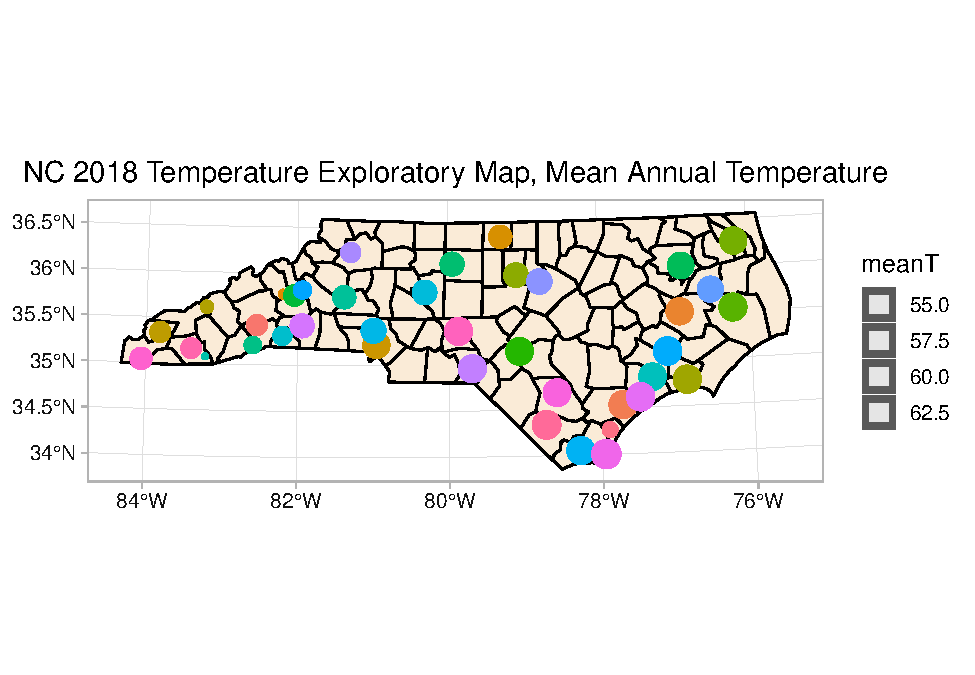
\includegraphics{./Outputunnamed-chunk-29-1.pdf}
\caption{Mean Annual Temperature exploratory map. \label{Tempplot}}
\end{figure}

\begin{figure}
\centering
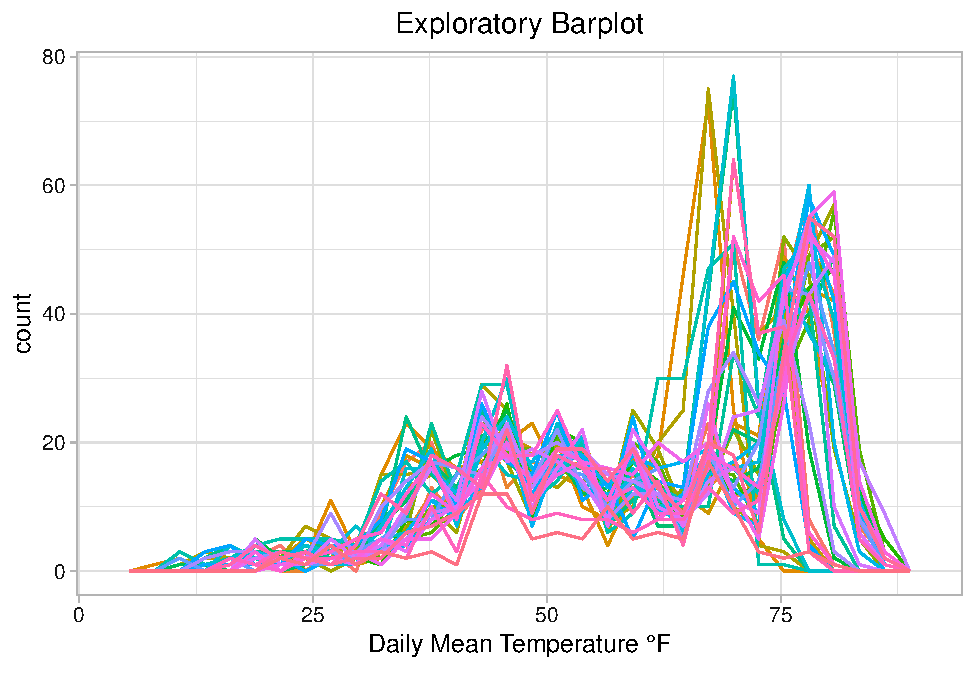
\includegraphics{./Outputunnamed-chunk-30-1.pdf}
\caption{Daily Mean Temperature NC 2018 frequency polygon.
\label{Temp_freqpoly}}
\end{figure}

\begin{figure}
\centering
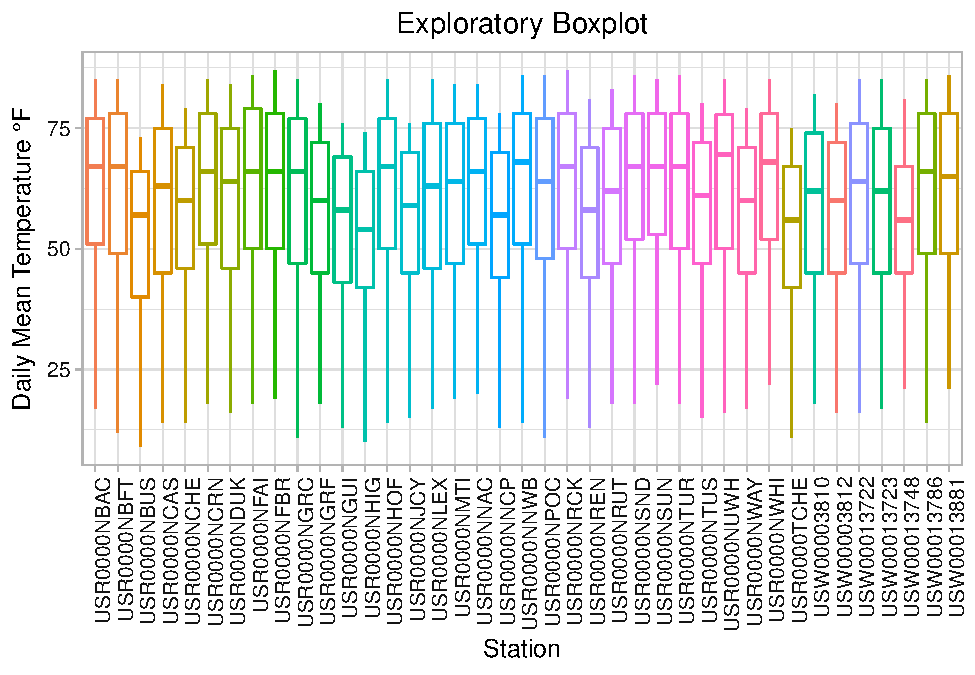
\includegraphics{./Outputunnamed-chunk-31-1.pdf}
\caption{Daily Mean Temperature NC 2018 boxplot. \label{Temp_boxplot}}
\end{figure}

\begin{figure}
\centering
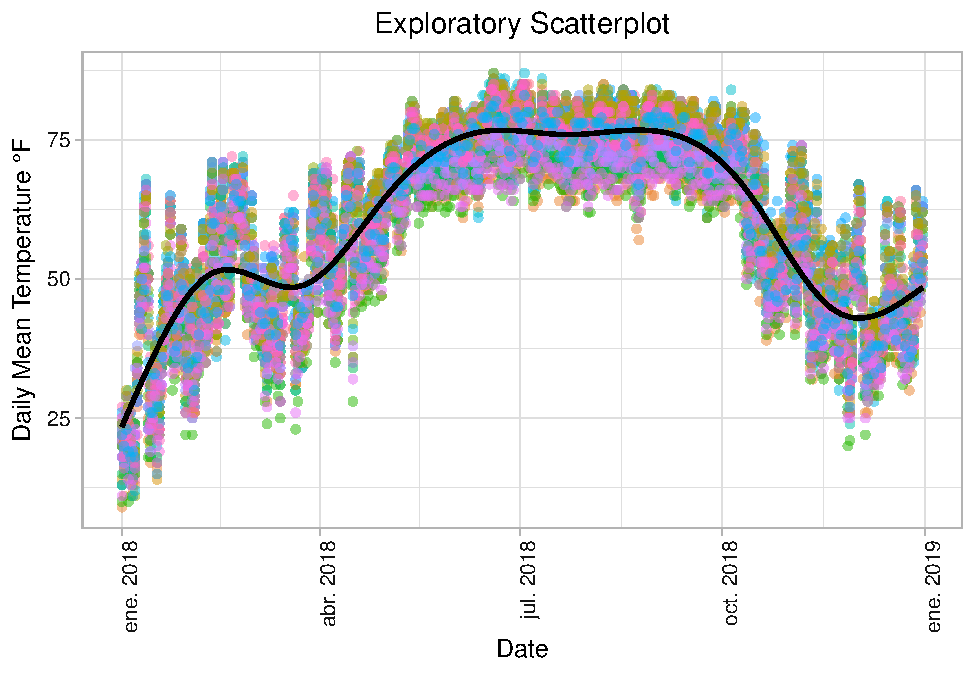
\includegraphics{./Outputunnamed-chunk-32-1.pdf}
\caption{Daily Mean Temperature NC 2018 scatterplot.
\label{Temp_scatterplot}}
\end{figure}

Next, the temperature of the nearest Temperature Station is added to
each PM2.5 Station in the PM2.5\_PM10\_Info\_sf\_utm dataframe.

\begin{Shaded}
\begin{Highlighting}[]
\CommentTok{#Create a Data frame with only the PM2.5 station info}
\NormalTok{PM2.5_Stations <-}\StringTok{ }\NormalTok{PM2.5_PM10_Info_sf_utm }\OperatorTok
\StringTok{  }\KeywordTok{select}\NormalTok{(Site.ID, geometry) }\OperatorTok
\StringTok{  }\KeywordTok{subset}\NormalTok{(}\OperatorTok{!}\KeywordTok{duplicated}\NormalTok{(Site.ID))}

\CommentTok{#Distances bewteen the PM2.5 stations and the Temperature Stations}
\NormalTok{Nearest <-}\StringTok{ }\KeywordTok{st_nearest_feature}\NormalTok{(PM2.5_Stations, NOAA_DTAVG_NC2018_sf_utm)}

\NormalTok{a <-}\StringTok{ }\KeywordTok{length}\NormalTok{(}\KeywordTok{unique}\NormalTok{(PM2.5_Stations}\OperatorTok{$}\NormalTok{Site.ID))}

\NormalTok{NOAA_DTAVG_NC2018_sf_utm}\OperatorTok{$}\NormalTok{NAME <-}\StringTok{ }\KeywordTok{as.character}\NormalTok{(NOAA_DTAVG_NC2018_sf_utm}\OperatorTok{$}\NormalTok{NAME)}

\CommentTok{#Assingning the nearest Temperature Station to each PM2.5 station.}
\ControlFlowTok{for}\NormalTok{ (i }\ControlFlowTok{in} \DecValTok{1}\OperatorTok{:}\NormalTok{a)\{}
\NormalTok{  PM2.5_Stations}\OperatorTok{$}\NormalTok{Temp_Est[i] <-}\StringTok{ }\NormalTok{NOAA_DTAVG_NC2018_sf_utm}\OperatorTok{$}\NormalTok{NAME[Nearest[i]]}
\NormalTok{\}}

\CommentTok{#Drop the geo data}
\NormalTok{aux2 <-}\StringTok{ }\KeywordTok{st_set_geometry}\NormalTok{(PM2.5_Stations, }\DataTypeTok{value=}\OtherTok{NULL}\NormalTok{)}

\CommentTok{#Left_join the data}
\NormalTok{PM2.5_PM10_Temp_sf_utm <-}\StringTok{ }\NormalTok{PM2.5_PM10_Info_sf_utm }\OperatorTok
\KeywordTok{left_join}\NormalTok{(aux2)}

\CommentTok{#Assingning the Temperature of the nearest Temperature Station to each PM2.5 station.}

\CommentTok{#Drops the geo data}
\NormalTok{aux3 <-}\StringTok{ }\KeywordTok{st_set_geometry}\NormalTok{(NOAA_DTAVG_NC2018_sf_utm, }\DataTypeTok{value=}\OtherTok{NULL}\NormalTok{)}

\CommentTok{#Left_join the data}
\NormalTok{PM2.5_PM10_Temp_sf_utm <-}\StringTok{ }\NormalTok{PM2.5_PM10_Temp_sf_utm }\OperatorTok
\KeywordTok{left_join}\NormalTok{(aux3, }\DataTypeTok{by =} \KeywordTok{c}\NormalTok{(}\StringTok{"Temp_Est"}\NormalTok{=}\StringTok{"NAME"}\NormalTok{, }\StringTok{"Date"}\NormalTok{=}\StringTok{"DATE"}\NormalTok{, }\StringTok{"COUNTY"}\NormalTok{)) }\OperatorTok
\StringTok{  }\KeywordTok{select}\NormalTok{(Date,Site.ID,COUNTY,Population,Zone,PM2.}\DecValTok{5}\NormalTok{,PM10,TAVG,geometry)}
\end{Highlighting}
\end{Shaded}

\subsection{EPA combustion points for electricity generation in the US
Dataset}\label{epa-combustion-points-for-electricity-generation-in-the-us-dataset-1}

Reading the Electricity Generation via Combustion data.

\begin{Shaded}
\begin{Highlighting}[]
\NormalTok{EPA_US_CombEmissions <-}\StringTok{ }\KeywordTok{st_read}\NormalTok{(}\StringTok{"./Data/Raw/EPA_ElecGenComb_US_raw.kml"}\NormalTok{)}
\end{Highlighting}
\end{Shaded}

\begin{verbatim}
## Reading layer `Electricity Generation via Combustion' from data source `C:\Users\Felipe\OneDrive - Duke University\1. DUKE\1. Ramos 2 Semestre\EOS-872 Env. Data Analytics\DataAnalytics_FinalProject\Data\Raw\EPA_ElecGenComb_US_raw.kml' using driver `KML'
## Simple feature collection with 2042 features and 2 fields
## geometry type:  POINT
## dimension:      XYZ
## bbox:           xmin: -176.6593 ymin: 19.63283 xmax: -67.00325 ymax: 71.29221
## epsg (SRID):    4326
## proj4string:    +proj=longlat +datum=WGS84 +no_defs
\end{verbatim}

Wrangling the data

\begin{Shaded}
\begin{Highlighting}[]
\KeywordTok{st_crs}\NormalTok{(EPA_US_CombEmissions) }\CommentTok{#crs=4326 = WGS 84}
\end{Highlighting}
\end{Shaded}

\begin{verbatim}
## Coordinate Reference System:
##   EPSG: 4326 
##   proj4string: "+proj=longlat +datum=WGS84 +no_defs"
\end{verbatim}

\begin{Shaded}
\begin{Highlighting}[]
\CommentTok{#Convert all to UTM Zone 17 (crs = 26917)}
\NormalTok{EPA_US_CombEmissions_utm <-}\StringTok{ }\KeywordTok{st_transform}\NormalTok{(EPA_US_CombEmissions, }\DataTypeTok{c=}\DecValTok{26917}\NormalTok{)}

\CommentTok{#Clip the EPA_US_CombEmissions data set by the NC State boundary dataset}

\CommentTok{#First create a State_sf file}
\CommentTok{#Aggregate the data using group_by and summarize, just as you would a non-spatial dataframe}
\NormalTok{state_sf_utm <-}\StringTok{ }\KeywordTok{st_union}\NormalTok{(counties_sf_utm)}

\CommentTok{#Eliminate the emission points outside NC}
\NormalTok{EPA_NC_CombEmissions_utm <-}\StringTok{ }\KeywordTok{st_intersection}\NormalTok{(EPA_US_CombEmissions_utm,state_sf_utm) }
\end{Highlighting}
\end{Shaded}

Visual data exploration of the EPA combustion points for electricity
generation in the North Carolina in \autoref{Tempplot},
\autoref{Temp_freqpoly}, \autoref{Combplot}, and
\autoref{Temp_scatterplot}..

\begin{figure}
\centering
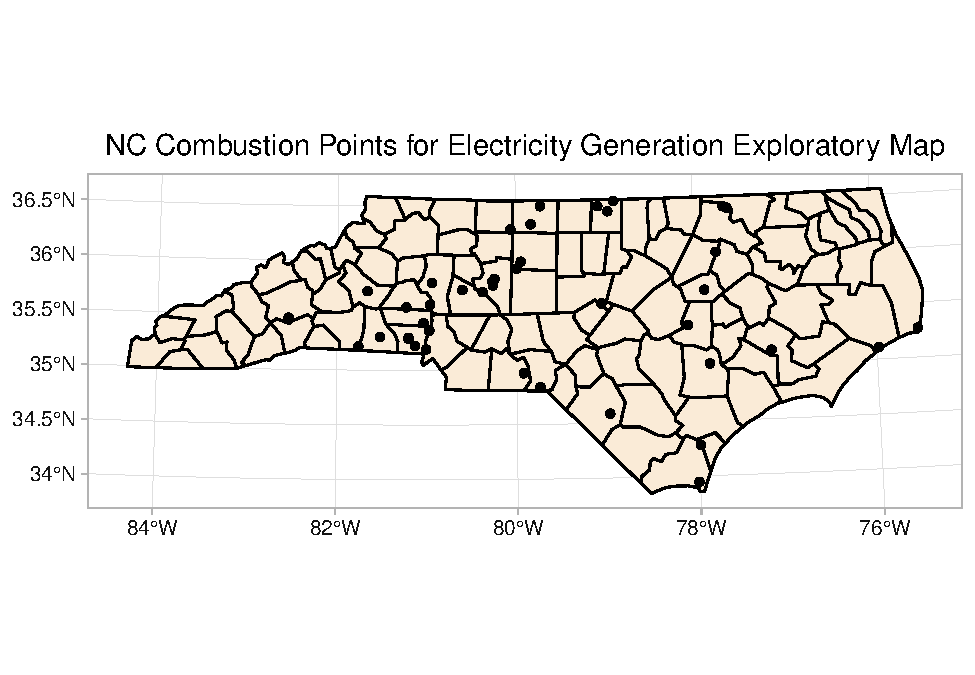
\includegraphics{./Outputunnamed-chunk-36-1.pdf}
\caption{Combustion points for electricity generation in the North
Carolina. \label{Combplot}}
\end{figure}

Now the distance between PM2.5 stations and Electricity Generation via
Combustion points is determined and added to the
PM2.5\_PM10\_Temp\_sf\_utm dataframe.

\begin{Shaded}
\begin{Highlighting}[]
\CommentTok{#Distances between PM2.5 stations and Electricity Generation via Combustion points}
\NormalTok{Distances <-}\StringTok{ }\KeywordTok{st_distance}\NormalTok{(PM2.5_Stations, EPA_NC_CombEmissions_utm)}

\NormalTok{a <-}\StringTok{ }\KeywordTok{length}\NormalTok{(}\KeywordTok{unique}\NormalTok{(PM2.5_Stations}\OperatorTok{$}\NormalTok{Site.ID))}

\CommentTok{#Determining the minimum distance of each PM2.5 station to a combustion point in meters.}
\ControlFlowTok{for}\NormalTok{ (i }\ControlFlowTok{in} \DecValTok{1}\OperatorTok{:}\NormalTok{a)\{}
\NormalTok{  PM2.5_Stations}\OperatorTok{$}\NormalTok{Emiss_Dist[i] <-}\StringTok{ }\KeywordTok{min}\NormalTok{(Distances[i,])}
\NormalTok{\}}

\CommentTok{#Filling the PM2.5_PM10_Temp_sf_utm file with the distances}

\CommentTok{#Drops the geo data}
\NormalTok{aux4 <-}\StringTok{ }\NormalTok{PM2.5_Stations }\OperatorTok
\StringTok{  }\KeywordTok{st_set_geometry}\NormalTok{(}\DataTypeTok{value=}\OtherTok{NULL}\NormalTok{) }\OperatorTok\StringTok{ }
\StringTok{  }\KeywordTok{select}\NormalTok{(Site.ID,Emiss_Dist)}

\CommentTok{#Left_join the data}
\NormalTok{PM2.5_Full_utm <-}\StringTok{ }\NormalTok{PM2.5_PM10_Temp_sf_utm }\OperatorTok
\KeywordTok{left_join}\NormalTok{(aux4, }\DataTypeTok{by =} \KeywordTok{c}\NormalTok{(}\StringTok{"Site.ID"}\NormalTok{)) }\OperatorTok
\StringTok{  }\KeywordTok{select}\NormalTok{(Date,Site.ID,COUNTY,Population,Zone,PM2.}\DecValTok{5}\NormalTok{,PM10,TAVG,Emiss_Dist,geometry)}
\end{Highlighting}
\end{Shaded}

Finally, using the elevatr package, elevation information is added to
the PM 2.5 stations in the PM2.5\_Full\_utm dataframe, creating the
PM2.5\_Full\_Elev\_utm, which is saved in the Project folder
./Data/Processed.

Elevations for the PM2.5 Stations

\begin{Shaded}
\begin{Highlighting}[]
\NormalTok{prj_dd <-}\StringTok{ "+proj=utm +zone=17 +ellps=GRS80 +towgs84=0,0,0,0,0,0,0 +units=m +no_defs"}
\NormalTok{PM2.5_Full_Elev_utm <-}\StringTok{ }\KeywordTok{get_elev_point}\NormalTok{(PM2.5_Full_utm, }\DataTypeTok{prj =}\NormalTok{ prj_dd, }\DataTypeTok{src =} \StringTok{"epqs"}\NormalTok{)}

\KeywordTok{st_write}\NormalTok{(PM2.5_Full_Elev_utm,}
         \StringTok{"./Data/Processed/PM2.5_Full_Elev_utm.shp"}\NormalTok{, }\DataTypeTok{driver =} \StringTok{"ESRI Shapefile"}\NormalTok{)}
\end{Highlighting}
\end{Shaded}

\begin{Shaded}
\begin{Highlighting}[]
\NormalTok{PM2.5_Full_Elev_utm <-}\StringTok{ }\KeywordTok{st_read}\NormalTok{(}\StringTok{'./Data/Processed/PM2.5_Full_Elev_utm.shp'}\NormalTok{) }
\end{Highlighting}
\end{Shaded}

\begin{verbatim}
## Reading layer `PM2.5_Full_Elev_utm' from data source `C:\Users\Felipe\OneDrive - Duke University\1. DUKE\1. Ramos 2 Semestre\EOS-872 Env. Data Analytics\DataAnalytics_FinalProject\Data\Processed\PM2.5_Full_Elev_utm.shp' using driver `ESRI Shapefile'
## Simple feature collection with 7460 features and 11 fields
## geometry type:  POINT
## dimension:      XY
## bbox:           xmin: 278314.3 ymin: 3807066 xmax: 935107.5 ymax: 3996703
## epsg (SRID):    NA
## proj4string:    +proj=utm +zone=17 +ellps=GRS80 +units=m +no_defs
\end{verbatim}

\subsection{Additional previsualization of the
data}\label{additional-previsualization-of-the-data}

\newpage

\section{Analysis}\label{analysis}

In 2012, the United States Environmental Protection Agency (USEPA)
established two complementary primary regulatory standards for PM2.5.
The first is based on a yearly average value and is set at 12 micrograms
per cubic meter, ug/m3,

First statistical test should look at the standard in each station.

FRA: This model structure should look familiar, with a typical linear
model structure and dataframe defined. The addition here is that we have
defined Week as a random variable. Essentially, we are interested not in
the specific effects of each week but in the variability among weeks, so
we have defined it as a random effect (essentially coming from a larger
distribution of seasonal variability).

\newpage

\section{Summary and Conclusions}\label{summary-and-conclusions}


\end{document}
